\chapter{Implementing Motors in Rigid Multibody Algorithms}
\label{chp:MotorDynamics}

This chapter describes the formalism and the algorithms involved in the conditioning of multibody systems behavior, taking into account motor dynamics in the framework of recursive computation methods. First, a mathematical groundwork for characterizing the dynamics of a floating-base multibody system is presented, setting a convention that is used throughout this work. Then, the problem of injecting motor parameters in the \ac{EoM} is discussed and finally the core implementation in recursive algorithms is argued.

\section{Mathematical Preliminaries}

In the forthcoming discussion, a 6D \textit{spatial vectors} notation firstly introduced by R. Featherstone \cite{featherstone_rigid_2008} is presented. This will be used to describe the kinematics and dynamics of a floating-base multibody system in a unified manner.

\paragraph{Spatial Vectors} A spatial vector is a 6D vector that describes the motion of a rigid body in space.

In the case of a rigid body, the velocity of a point $P$ attached to the body respect to a reference frame attached to an arbitrary point $O$ in the space can be generally expressed by its angular component $\mathbf{\omega}$ about an axis passing through $O$ and its linear component $\mathbf{v} _P$, for which the following relation holds:

\begin{equation}
    v _P = \mathbf{\omega} \times \bar{OP}
\end{equation}

where $\bar{OP}$ is the position vector of $P$ with respect to $O$. This holds for any point $P$ on the rigid body. In order to simplify the notation, introducing a Cartesian coordinate frame $\mathcal{O} _{xyz}$, we can define a basis of 6 spatial vectors $\mathcal{D} _O = \{\mathbf{d} _i\} ^6 _{i=1}$ as:

\begin{equation}
    \mathcal{D} _O = \{ \mathbf{d} _{O _x}, \mathbf{d} _{O _y}, \mathbf{d} _{O _z}, \mathbf{d} _x, \mathbf{d} _y, \mathbf{d} _z \} \subset \mathcal{M} ^6
\end{equation}

where $\mathcal{M} ^6$ is the space of 6D vectors, defining a Pl\"ucker coordinate system on $\mathcal{M} ^6$.


\dots

\paragraph{Spatial Velocity} \dots The spatial velocity of a rigid body is defined as:

\begin{equation}
    \mathbf{v} _P = \begin{bmatrix}
        \mathbf{v} _P \\
        \boldsymbol{\omega} _P
    \end{bmatrix}
\end{equation}

where $\mathbf{v} _P$ is the linear velocity of the point $P$ and $\boldsymbol{\omega} _P$ is the angular velocity of the body.

\paragraph{Spatial Forces} \dots The spatial force acting on a rigid body is defined as:

\begin{equation}
    \mathbf{f} = \begin{bmatrix}
        \mathbf{f} \\
        \boldsymbol{\tau}
    \end{bmatrix}
\end{equation}



\section{Problem Formalization}

Starting from the equation of motion of a robot manipulator:

\begin{equation}
    \mathbf{M}(q)\dot{\boldsymbol{\nu}} + \mathbf{h}(q,\boldsymbol{\nu}) = \mathbf{B}\boldsymbol{\tau} + \mathbf{J} ^T \mathbf{f}
\end{equation}

where:

\begin{itemize}
    \item $\mathbf{M}(q)$ is the inertia matrix
    \item $\mathbf{h}(q,\boldsymbol{\nu})$ is the Coriolis vector
    \item $\mathbf{B}$ is the actuation matrix
    \item $\boldsymbol{\tau}$ is actuation torques vector
    \item $\mathbf{J}$ is the Jacobian matrix
    \item $\mathbf{f}$ is the external forces vector
\end{itemize}

we can isolate the terms related to the base link (usually in position 0) from the joints' poses:

\begin{align}
    \boldsymbol{\nu} =
    \begin{bmatrix}
        \mathrm{\mathbf{v}} \\
        \dot{\mathbf{s}}
    \end{bmatrix} &  &
    \dot{\boldsymbol{\nu}} =
    \begin{bmatrix}
        \dot{\mathrm{\mathbf{v}}} \\
        \ddot{\mathbf{s}}
    \end{bmatrix}
\end{align}

where $\mathrm{\mathbf{v}} \in \mathbb{R} ^{6}$ and $\mathbf{s} \in \mathbb{R}^{N_B}$, we get to the form:

\begin{equation}
    \begin{bmatrix}
        \mathbf{M} _{\mathcal{B}}(q)     & \mathbf{M} _{\mathcal{B}S}(q) \\
        \mathbf{M} _{\mathcal{B}S} ^T(q) & \mathbf{M} _s(q)
    \end{bmatrix}
    \begin{bmatrix}
        \dot{\mathrm{\mathbf{v}}} \\
        \ddot{\mathbf{s}}
    \end{bmatrix}+
    \begin{bmatrix}
        \mathbf{h} _{\mathcal{B}} \\
        \mathbf{h} _S
    \end{bmatrix}=
    \begin{bmatrix}
        \mathbb{0} \\
        \mathbb{1}
    \end{bmatrix}
    \boldsymbol{\tau}
    +
    \begin{bmatrix}
        \mathbf{J} _{\mathcal{B}} \\
        \mathbf{J} _S
    \end{bmatrix} ^T
    \mathbf{f}
\end{equation}

Given that the dynamics of the set of motors can be described by the following equation:

\begin{equation}
    \label{eqn:mot_dyn}
    \mathbf{I} _R \ddot{\boldsymbol{\theta}} + \mathbf{K}_v \dot{\boldsymbol{\theta}} = \boldsymbol{\tau}_m
\end{equation}

where $\mathbf{K _v}$ is the diagonal matrix of motor viscous coefficients and $\mathbf{I}_R$ is the diagonal matrix of motors' inertias. Considering that given the set of transmission ratios $\boldsymbol{\Gamma}$, the relation between the joints' velocities and the motors' velocities is:

\begin{align}
    \mathbf{s} = \boldsymbol{\theta} \boldsymbol{\Gamma} &  & \dot{\mathbf{s}} = \dot{\boldsymbol{\theta}} \boldsymbol{\Gamma} &  & \ddot{\mathbf{s}} = \ddot{\boldsymbol{\theta}} \boldsymbol{\Gamma}
\end{align}

we can rewrite the equation \ref{eqn:mot_dyn} in the joints' space as:

\begin{equation}
    \label{eqn:mot_dyn_jointspace}
    \boldsymbol{\tau} = \boldsymbol{\Gamma} ^{-T} (\mathbf{I} _R\boldsymbol{\Gamma} ^{-1} \ddot{s} + \mathbf{K}_v \boldsymbol{\Gamma} ^{-1}\dot{s})
\end{equation}

Therefore, the \ac{EoM} of the multibody system can be rewritten as:

\begin{equation}
    \underbrace{\begin{bmatrix}
            \mathbf{M} _{\mathcal{B}}(q)     & \mathbf{M} _{\mathcal{B}S}(q)                                                      \\
            \mathbf{M} _{\mathcal{B}S} ^T(q) & \mathbf{M} _s(q) + \boldsymbol{\Gamma} ^{-T}\mathbf{I} _R\boldsymbol{\Gamma} ^{-1}
        \end{bmatrix}} _{\mathbf{\bar{M}}(q)}
    \begin{bmatrix}
        \dot{\mathrm{\mathbf{v}}} \\
        \ddot{\mathbf{s}}
    \end{bmatrix}+
    \mathbf{h}
    (q,\boldsymbol{\nu}) =
    \underbrace{\begin{bmatrix}
            \mathbb{0} \\
            \boldsymbol{\Gamma} ^{-T}
        \end{bmatrix}} _{\mathbf{\bar{B}}}
    \boldsymbol{\tau} _m
    +
    \mathbf{J} ^T
    \mathbf{f}
    -
    \underbrace{\begin{bmatrix}
            \mathbb{0} \\
            \boldsymbol{\Gamma} ^{-T}\mathbf{K _v}\boldsymbol{\Gamma} ^{-1}
        \end{bmatrix}} _\mathbf{\bar{K _v}}
    \begin{bmatrix}
        \mathrm{\mathbf{v}} \\
        \dot{\mathbf{s}}
    \end{bmatrix}
\end{equation}

or, in a more compact form that will be used for computation as:

\begin{equation}
    \mathbf{\bar{M}}(q)\dot{\boldsymbol{\nu}} + \mathbf{h}(q,\boldsymbol{\nu}) = \mathbf{\bar{B}}\boldsymbol{\tau} _m + \mathbf{J} ^T \mathbf{f} - \bar{\mathbf{K _v}}\boldsymbol{\nu}
\end{equation}

\subsection{Articulated Body Algorithm}

% === FIG: Kynematic Chain === %
\begin{figure}[h]
    \centering
    \label{fig:kin_tree}
    \caption{Branched kinematic tree}
    \tikzset {_wvafpciex/.code = {\pgfsetadditionalshadetransform{ \pgftransformshift{\pgfpoint{0 bp } { 0 bp }  }  \pgftransformrotate{-117 }  \pgftransformscale{2 }  }}}
    \pgfdeclarehorizontalshading{_sy15ycl19}{150bp}{rgb(0bp)=(1,1,1);
        rgb(37.5bp)=(1,1,1);
        rgb(50.08184160505022bp)=(0.95,0.95,0.95);
        rgb(57.64583042689732bp)=(0.88,0.88,0.88);
        rgb(61.33184160505022bp)=(0.96,0.96,0.96);
        rgb(100bp)=(0.96,0.96,0.96)}
    \tikzset {_svf4mjzjm/.code = {\pgfsetadditionalshadetransform{ \pgftransformshift{\pgfpoint{0 bp } { 0 bp }  }  \pgftransformrotate{-117 }  \pgftransformscale{2 }  }}}
    \pgfdeclarehorizontalshading{_e9qihdtow}{150bp}{rgb(0bp)=(1,1,1);
        rgb(37.5bp)=(1,1,1);
        rgb(50.08184160505022bp)=(0.95,0.95,0.95);
        rgb(57.64583042689732bp)=(0.88,0.88,0.88);
        rgb(61.33184160505022bp)=(0.96,0.96,0.96);
        rgb(100bp)=(0.96,0.96,0.96)}
    \tikzset {_ddhli8fcf/.code = {\pgfsetadditionalshadetransform{ \pgftransformshift{\pgfpoint{0 bp } { 0 bp }  }  \pgftransformrotate{-117 }  \pgftransformscale{2 }  }}}
    \pgfdeclarehorizontalshading{_bw97u0oo5}{150bp}{rgb(0bp)=(1,1,1);
        rgb(37.5bp)=(1,1,1);
        rgb(50.08184160505022bp)=(0.95,0.95,0.95);
        rgb(57.64583042689732bp)=(0.88,0.88,0.88);
        rgb(61.33184160505022bp)=(0.96,0.96,0.96);
        rgb(100bp)=(0.96,0.96,0.96)}
    \tikzset {_rzri9nu6o/.code = {\pgfsetadditionalshadetransform{ \pgftransformshift{\pgfpoint{0 bp } { 0 bp }  }  \pgftransformrotate{-117 }  \pgftransformscale{2 }  }}}
    \pgfdeclarehorizontalshading{_irmxrz6bl}{150bp}{rgb(0bp)=(1,1,1);
        rgb(37.5bp)=(1,1,1);
        rgb(50.08184160505022bp)=(0.95,0.95,0.95);
        rgb(57.64583042689732bp)=(0.88,0.88,0.88);
        rgb(61.33184160505022bp)=(0.96,0.96,0.96);
        rgb(100bp)=(0.96,0.96,0.96)}
    \tikzset {_tv3cr0nbo/.code = {\pgfsetadditionalshadetransform{ \pgftransformshift{\pgfpoint{0 bp } { 0 bp }  }  \pgftransformrotate{-117 }  \pgftransformscale{2 }  }}}
    \pgfdeclarehorizontalshading{_ria03yqfs}{150bp}{rgb(0bp)=(1,1,1);
        rgb(37.5bp)=(1,1,1);
        rgb(50.08184160505022bp)=(0.95,0.95,0.95);
        rgb(57.64583042689732bp)=(0.88,0.88,0.88);
        rgb(61.33184160505022bp)=(0.96,0.96,0.96);
        rgb(100bp)=(0.96,0.96,0.96)}
    \tikzset {_0hgwncxm6/.code = {\pgfsetadditionalshadetransform{ \pgftransformshift{\pgfpoint{0 bp } { 0 bp }  }  \pgftransformrotate{-117 }  \pgftransformscale{2 }  }}}
    \pgfdeclarehorizontalshading{_7fixrohbn}{150bp}{rgb(0bp)=(1,1,1);
        rgb(37.5bp)=(1,1,1);
        rgb(50.08184160505022bp)=(0.95,0.95,0.95);
        rgb(57.64583042689732bp)=(0.88,0.88,0.88);
        rgb(61.33184160505022bp)=(0.96,0.96,0.96);
        rgb(100bp)=(0.96,0.96,0.96)}
    \tikzset {_te42shfqc/.code = {\pgfsetadditionalshadetransform{ \pgftransformshift{\pgfpoint{0 bp } { 0 bp }  }  \pgftransformrotate{-117 }  \pgftransformscale{2 }  }}}
    \pgfdeclarehorizontalshading{_9prsrmsl7}{150bp}{rgb(0bp)=(1,1,1);
        rgb(37.5bp)=(1,1,1);
        rgb(50.08184160505022bp)=(0.95,0.95,0.95);
        rgb(57.64583042689732bp)=(0.88,0.88,0.88);
        rgb(61.33184160505022bp)=(0.96,0.96,0.96);
        rgb(100bp)=(0.96,0.96,0.96)}
    \tikzset {_qoggn7fn2/.code = {\pgfsetadditionalshadetransform{ \pgftransformshift{\pgfpoint{0 bp } { 0 bp }  }  \pgftransformrotate{-117 }  \pgftransformscale{2 }  }}}
    \pgfdeclarehorizontalshading{_8g14z78sd}{150bp}{rgb(0bp)=(1,1,1);
        rgb(37.5bp)=(1,1,1);
        rgb(50.08184160505022bp)=(0.95,0.95,0.95);
        rgb(57.64583042689732bp)=(0.88,0.88,0.88);
        rgb(61.33184160505022bp)=(0.96,0.96,0.96);
        rgb(100bp)=(0.96,0.96,0.96)}
    \tikzset {_3ytgx3jcr/.code = {\pgfsetadditionalshadetransform{ \pgftransformshift{\pgfpoint{0 bp } { 0 bp }  }  \pgftransformrotate{-117 }  \pgftransformscale{2 }  }}}
    \pgfdeclarehorizontalshading{_hjawm1m3k}{150bp}{rgb(0bp)=(1,1,1);
        rgb(37.5bp)=(1,1,1);
        rgb(50.08184160505022bp)=(0.95,0.95,0.95);
        rgb(57.64583042689732bp)=(0.88,0.88,0.88);
        rgb(61.33184160505022bp)=(0.96,0.96,0.96);
        rgb(100bp)=(0.96,0.96,0.96)}
    \tikzset {_pm47npqyx/.code = {\pgfsetadditionalshadetransform{ \pgftransformshift{\pgfpoint{0 bp } { 0 bp }  }  \pgftransformrotate{-117 }  \pgftransformscale{2 }  }}}
    \pgfdeclarehorizontalshading{_hbtcw454n}{150bp}{rgb(0bp)=(1,1,1);
        rgb(37.5bp)=(1,1,1);
        rgb(50.08184160505022bp)=(0.95,0.95,0.95);
        rgb(57.64583042689732bp)=(0.88,0.88,0.88);
        rgb(61.33184160505022bp)=(0.96,0.96,0.96);
        rgb(100bp)=(0.96,0.96,0.96)}
    \tikzset {_igkxxgbt5/.code = {\pgfsetadditionalshadetransform{ \pgftransformshift{\pgfpoint{0 bp } { 0 bp }  }  \pgftransformrotate{-117 }  \pgftransformscale{2 }  }}}
    \pgfdeclarehorizontalshading{_4ks716t6n}{150bp}{rgb(0bp)=(1,1,1);
        rgb(37.5bp)=(1,1,1);
        rgb(50.08184160505022bp)=(0.95,0.95,0.95);
        rgb(57.64583042689732bp)=(0.88,0.88,0.88);
        rgb(61.33184160505022bp)=(0.96,0.96,0.96);
        rgb(100bp)=(0.96,0.96,0.96)}
    \tikzset{every picture/.style={line width=0.75pt}}
    \begin{tikzpicture}[x=0.75pt,y=0.75pt,yscale=-1,xscale=1]
        \path  [shading=_sy15ycl19,_wvafpciex] (340.92,97.33) .. controls (340.92,88.96) and (364.78,82.17) .. (394.21,82.17) .. controls (423.64,82.17) and (447.5,88.96) .. (447.5,97.33) .. controls (447.5,105.71) and (423.64,112.5) .. (394.21,112.5) .. controls (364.78,112.5) and (340.92,105.71) .. (340.92,97.33) -- cycle ; % for fading 
        \draw  [color={rgb, 255:red, 0; green, 0; blue, 0 }  ,draw opacity=1 ][line width=0.75]  (340.92,97.33) .. controls (340.92,88.96) and (364.78,82.17) .. (394.21,82.17) .. controls (423.64,82.17) and (447.5,88.96) .. (447.5,97.33) .. controls (447.5,105.71) and (423.64,112.5) .. (394.21,112.5) .. controls (364.78,112.5) and (340.92,105.71) .. (340.92,97.33) -- cycle ; % for border 
        \path  [shading=_e9qihdtow,_svf4mjzjm] (528.22,14.11) .. controls (534.45,19.72) and (523.53,41.99) .. (503.84,63.87) .. controls (484.15,85.75) and (463.14,98.94) .. (456.92,93.33) .. controls (450.69,87.73) and (461.61,65.45) .. (481.3,43.58) .. controls (500.99,21.7) and (522,8.51) .. (528.22,14.11) -- cycle ; % for fading 
        \draw  [color={rgb, 255:red, 0; green, 0; blue, 0 }  ,draw opacity=1 ][line width=0.75]  (528.22,14.11) .. controls (534.45,19.72) and (523.53,41.99) .. (503.84,63.87) .. controls (484.15,85.75) and (463.14,98.94) .. (456.92,93.33) .. controls (450.69,87.73) and (461.61,65.45) .. (481.3,43.58) .. controls (500.99,21.7) and (522,8.51) .. (528.22,14.11) -- cycle ; % for border 
        \path  [shading=_bw97u0oo5,_ddhli8fcf] (447.5,97.33) .. controls (447.5,94.46) and (449.83,92.13) .. (452.71,92.13) .. controls (455.58,92.13) and (457.92,94.46) .. (457.92,97.33) .. controls (457.92,100.21) and (455.58,102.54) .. (452.71,102.54) .. controls (449.83,102.54) and (447.5,100.21) .. (447.5,97.33) -- cycle ; % for fading 
        \draw  [color={rgb, 255:red, 0; green, 0; blue, 0 }  ,draw opacity=1 ][line width=0.75]  (447.5,97.33) .. controls (447.5,94.46) and (449.83,92.13) .. (452.71,92.13) .. controls (455.58,92.13) and (457.92,94.46) .. (457.92,97.33) .. controls (457.92,100.21) and (455.58,102.54) .. (452.71,102.54) .. controls (449.83,102.54) and (447.5,100.21) .. (447.5,97.33) -- cycle ; % for border 
        \path  [shading=_irmxrz6bl,_rzri9nu6o] (332.22,101.61) .. controls (338.45,107.22) and (327.53,129.49) .. (307.84,151.37) .. controls (288.15,173.25) and (267.14,186.44) .. (260.92,180.83) .. controls (254.69,175.23) and (265.61,152.95) .. (285.3,131.08) .. controls (304.99,109.2) and (326,96.01) .. (332.22,101.61) -- cycle ; % for fading 
        \draw  [color={rgb, 255:red, 0; green, 0; blue, 0 }  ,draw opacity=1 ][line width=0.75]  (332.22,101.61) .. controls (338.45,107.22) and (327.53,129.49) .. (307.84,151.37) .. controls (288.15,173.25) and (267.14,186.44) .. (260.92,180.83) .. controls (254.69,175.23) and (265.61,152.95) .. (285.3,131.08) .. controls (304.99,109.2) and (326,96.01) .. (332.22,101.61) -- cycle ; % for border 
        \path  [shading=_ria03yqfs,_tv3cr0nbo] (330.5,97.33) .. controls (330.5,94.46) and (332.83,92.13) .. (335.71,92.13) .. controls (338.58,92.13) and (340.92,94.46) .. (340.92,97.33) .. controls (340.92,100.21) and (338.58,102.54) .. (335.71,102.54) .. controls (332.83,102.54) and (330.5,100.21) .. (330.5,97.33) -- cycle ; % for fading 
        \draw  [color={rgb, 255:red, 0; green, 0; blue, 0 }  ,draw opacity=1 ][line width=0.75]  (330.5,97.33) .. controls (330.5,94.46) and (332.83,92.13) .. (335.71,92.13) .. controls (338.58,92.13) and (340.92,94.46) .. (340.92,97.33) .. controls (340.92,100.21) and (338.58,102.54) .. (335.71,102.54) .. controls (332.83,102.54) and (330.5,100.21) .. (330.5,97.33) -- cycle ; % for border 
        \path  [shading=_7fixrohbn,_0hgwncxm6] (252.46,184.96) .. controls (252.46,182.08) and (254.79,179.75) .. (257.67,179.75) .. controls (260.54,179.75) and (262.87,182.08) .. (262.87,184.96) .. controls (262.87,187.83) and (260.54,190.17) .. (257.67,190.17) .. controls (254.79,190.17) and (252.46,187.83) .. (252.46,184.96) -- cycle ; % for fading 
        \draw  [color={rgb, 255:red, 0; green, 0; blue, 0 }  ,draw opacity=1 ][line width=0.75]  (252.46,184.96) .. controls (252.46,182.08) and (254.79,179.75) .. (257.67,179.75) .. controls (260.54,179.75) and (262.87,182.08) .. (262.87,184.96) .. controls (262.87,187.83) and (260.54,190.17) .. (257.67,190.17) .. controls (254.79,190.17) and (252.46,187.83) .. (252.46,184.96) -- cycle ; % for border 
        \path  [shading=_9prsrmsl7,_te42shfqc] (150.95,123.93) .. controls (143.63,128.01) and (126.08,110.48) .. (111.74,84.78) .. controls (97.4,59.08) and (91.7,34.93) .. (99.02,30.85) .. controls (106.33,26.77) and (123.89,44.3) .. (138.23,70) .. controls (152.57,95.7) and (158.26,119.85) .. (150.95,123.93) -- cycle ; % for fading 
        \draw  [color={rgb, 255:red, 0; green, 0; blue, 0 }  ,draw opacity=1 ][line width=0.75]  (150.95,123.93) .. controls (143.63,128.01) and (126.08,110.48) .. (111.74,84.78) .. controls (97.4,59.08) and (91.7,34.93) .. (99.02,30.85) .. controls (106.33,26.77) and (123.89,44.3) .. (138.23,70) .. controls (152.57,95.7) and (158.26,119.85) .. (150.95,123.93) -- cycle ; % for border 
        \path  [shading=_8g14z78sd,_qoggn7fn2] (159.33,130.95) .. controls (163.31,123.58) and (187.53,128.94) .. (213.43,142.93) .. controls (239.32,156.91) and (257.09,174.22) .. (253.11,181.59) .. controls (249.13,188.96) and (224.91,183.6) .. (199.01,169.62) .. controls (173.12,155.63) and (155.35,138.32) .. (159.33,130.95) -- cycle ; % for fading 
        \draw  [color={rgb, 255:red, 0; green, 0; blue, 0 }  ,draw opacity=1 ][line width=0.75]  (159.33,130.95) .. controls (163.31,123.58) and (187.53,128.94) .. (213.43,142.93) .. controls (239.32,156.91) and (257.09,174.22) .. (253.11,181.59) .. controls (249.13,188.96) and (224.91,183.6) .. (199.01,169.62) .. controls (173.12,155.63) and (155.35,138.32) .. (159.33,130.95) -- cycle ; % for border 
        \path  [shading=_hjawm1m3k,_3ytgx3jcr] (154.79,133.61) .. controls (151.92,133.71) and (149.51,131.45) .. (149.42,128.58) .. controls (149.32,125.7) and (151.58,123.3) .. (154.45,123.2) .. controls (157.33,123.11) and (159.73,125.36) .. (159.83,128.24) .. controls (159.92,131.11) and (157.67,133.52) .. (154.79,133.61) -- cycle ; % for fading 
        \draw  [color={rgb, 255:red, 0; green, 0; blue, 0 }  ,draw opacity=1 ][line width=0.75]  (154.79,133.61) .. controls (151.92,133.71) and (149.51,131.45) .. (149.42,128.58) .. controls (149.32,125.7) and (151.58,123.3) .. (154.45,123.2) .. controls (157.33,123.11) and (159.73,125.36) .. (159.83,128.24) .. controls (159.92,131.11) and (157.67,133.52) .. (154.79,133.61) -- cycle ; % for border 
        \path  [shading=_hbtcw454n,_pm47npqyx] (520.88,186.7) .. controls (514.23,191.8) and (494.33,176.98) .. (476.44,153.61) .. controls (458.55,130.24) and (449.43,107.17) .. (456.09,102.08) .. controls (462.74,96.98) and (482.63,111.8) .. (500.53,135.17) .. controls (518.42,158.54) and (527.53,181.61) .. (520.88,186.7) -- cycle ; % for fading 
        \draw  [color={rgb, 255:red, 0; green, 0; blue, 0 }  ,draw opacity=1 ][line width=0.75]  (520.88,186.7) .. controls (514.23,191.8) and (494.33,176.98) .. (476.44,153.61) .. controls (458.55,130.24) and (449.43,107.17) .. (456.09,102.08) .. controls (462.74,96.98) and (482.63,111.8) .. (500.53,135.17) .. controls (518.42,158.54) and (527.53,181.61) .. (520.88,186.7) -- cycle ; % for border 
        \path  [shading=_4ks716t6n,_igkxxgbt5] (225.88,232.5) .. controls (224.09,228.89) and (223.1,224.93) .. (223.1,220.77) .. controls (223.1,204.2) and (238.77,190.77) .. (258.1,190.77) .. controls (277.43,190.77) and (293.1,204.2) .. (293.1,220.77) .. controls (293.1,224.93) and (292.11,228.89) .. (290.32,232.5) -- cycle ; % for fading 
        \draw   (225.88,232.5) .. controls (224.09,228.89) and (223.1,224.93) .. (223.1,220.77) .. controls (223.1,204.2) and (238.77,190.77) .. (258.1,190.77) .. controls (277.43,190.77) and (293.1,204.2) .. (293.1,220.77) .. controls (293.1,224.93) and (292.11,228.89) .. (290.32,232.5) -- cycle ; % for border 
        \draw [color={rgb, 255:red, 0; green, 0; blue, 0 }  ,draw opacity=0.5 ]   (226.38,232.5) -- (233.96,240.33) ;
        \draw [color={rgb, 255:red, 0; green, 0; blue, 0 }  ,draw opacity=0.5 ]   (288.82,232.5) -- (296.41,240.33) ;
        \draw [color={rgb, 255:red, 0; green, 0; blue, 0 }  ,draw opacity=0.5 ]   (231.63,232.5) -- (239.21,240.33) ;
        \draw [color={rgb, 255:red, 0; green, 0; blue, 0 }  ,draw opacity=0.5 ]   (236.63,232.25) -- (244.21,240.08) ;
        \draw [color={rgb, 255:red, 0; green, 0; blue, 0 }  ,draw opacity=0.5 ]   (241.88,232.25) -- (249.46,240.08) ;
        \draw [color={rgb, 255:red, 0; green, 0; blue, 0 }  ,draw opacity=0.5 ]   (246.88,232.25) -- (254.46,240.08) ;
        \draw [color={rgb, 255:red, 0; green, 0; blue, 0 }  ,draw opacity=0.5 ]   (252.13,232.25) -- (259.71,240.08) ;
        \draw [color={rgb, 255:red, 0; green, 0; blue, 0 }  ,draw opacity=0.5 ]   (257.13,232.25) -- (264.71,240.08) ;
        \draw [color={rgb, 255:red, 0; green, 0; blue, 0 }  ,draw opacity=0.5 ]   (262.38,232.25) -- (269.96,240.08) ;
        \draw [color={rgb, 255:red, 0; green, 0; blue, 0 }  ,draw opacity=0.5 ]   (267.88,232.25) -- (275.46,240.08) ;
        \draw [color={rgb, 255:red, 0; green, 0; blue, 0 }  ,draw opacity=0.5 ]   (273.13,232.25) -- (280.71,240.08) ;
        \draw [color={rgb, 255:red, 0; green, 0; blue, 0 }  ,draw opacity=0.5 ]   (278.38,232.25) -- (285.96,240.08) ;
        \draw [color={rgb, 255:red, 0; green, 0; blue, 0 }  ,draw opacity=0.5 ]   (283.63,232.25) -- (291.21,240.08) ;
    \end{tikzpicture}
\end{figure}

% === FIG: Subtree === %
\begin{figure}
    \centering
    \caption{Kinematic subtree visualization.}
    \label{fig:subtree}
    \tikzset {_j7xuj04w0/.code = {\pgfsetadditionalshadetransform{ \pgftransformshift{\pgfpoint{0 bp } { 0 bp }  }  \pgftransformrotate{-117 }  \pgftransformscale{2 }  }}}
    \pgfdeclarehorizontalshading{_9jgwi88kk}{150bp}{rgb(0bp)=(1,1,1);
        rgb(37.5bp)=(1,1,1);
        rgb(50.08184160505022bp)=(0.95,0.95,0.95);
        rgb(57.64583042689732bp)=(0.88,0.88,0.88);
        rgb(61.33184160505022bp)=(0.96,0.96,0.96);
        rgb(100bp)=(0.96,0.96,0.96)}
    \tikzset {_i29mdsrh8/.code = {\pgfsetadditionalshadetransform{ \pgftransformshift{\pgfpoint{0 bp } { 0 bp }  }  \pgftransformrotate{-117 }  \pgftransformscale{2 }  }}}
    \pgfdeclarehorizontalshading{_4upvn6zpe}{150bp}{rgb(0bp)=(1,1,1);
        rgb(37.5bp)=(1,1,1);
        rgb(50.08184160505022bp)=(0.95,0.95,0.95);
        rgb(57.64583042689732bp)=(0.88,0.88,0.88);
        rgb(61.33184160505022bp)=(0.96,0.96,0.96);
        rgb(100bp)=(0.96,0.96,0.96)}
    \tikzset {_qh2wfjpes/.code = {\pgfsetadditionalshadetransform{ \pgftransformshift{\pgfpoint{0 bp } { 0 bp }  }  \pgftransformrotate{-117 }  \pgftransformscale{2 }  }}}
    \pgfdeclarehorizontalshading{_feqyochyi}{150bp}{rgb(0bp)=(1,1,1);
        rgb(37.5bp)=(1,1,1);
        rgb(50.08184160505022bp)=(0.95,0.95,0.95);
        rgb(57.64583042689732bp)=(0.88,0.88,0.88);
        rgb(61.33184160505022bp)=(0.96,0.96,0.96);
        rgb(100bp)=(0.96,0.96,0.96)}
    \tikzset {_d10v6gqbc/.code = {\pgfsetadditionalshadetransform{ \pgftransformshift{\pgfpoint{0 bp } { 0 bp }  }  \pgftransformrotate{-117 }  \pgftransformscale{2 }  }}}
    \pgfdeclarehorizontalshading{_gk602o946}{150bp}{rgb(0bp)=(1,1,1);
        rgb(37.5bp)=(1,1,1);
        rgb(50.08184160505022bp)=(0.95,0.95,0.95);
        rgb(57.64583042689732bp)=(0.88,0.88,0.88);
        rgb(61.33184160505022bp)=(0.96,0.96,0.96);
        rgb(100bp)=(0.96,0.96,0.96)}
    \tikzset {_8lna51u6m/.code = {\pgfsetadditionalshadetransform{ \pgftransformshift{\pgfpoint{0 bp } { 0 bp }  }  \pgftransformrotate{-117 }  \pgftransformscale{2 }  }}}
    \pgfdeclarehorizontalshading{_l87ke29nk}{150bp}{rgb(0bp)=(1,1,1);
        rgb(37.5bp)=(1,1,1);
        rgb(50.08184160505022bp)=(0.95,0.95,0.95);
        rgb(57.64583042689732bp)=(0.88,0.88,0.88);
        rgb(61.33184160505022bp)=(0.96,0.96,0.96);
        rgb(100bp)=(0.96,0.96,0.96)}
    \tikzset {_flvzdphcz/.code = {\pgfsetadditionalshadetransform{ \pgftransformshift{\pgfpoint{0 bp } { 0 bp }  }  \pgftransformrotate{-117 }  \pgftransformscale{2 }  }}}
    \pgfdeclarehorizontalshading{_5rkeipgwd}{150bp}{rgb(0bp)=(1,1,1);
        rgb(37.5bp)=(1,1,1);
        rgb(50.08184160505022bp)=(0.95,0.95,0.95);
        rgb(57.64583042689732bp)=(0.88,0.88,0.88);
        rgb(61.33184160505022bp)=(0.96,0.96,0.96);
        rgb(100bp)=(0.96,0.96,0.96)}
    \tikzset {_lvfzf5nu3/.code = {\pgfsetadditionalshadetransform{ \pgftransformshift{\pgfpoint{0 bp } { 0 bp }  }  \pgftransformrotate{-117 }  \pgftransformscale{2 }  }}}
    \pgfdeclarehorizontalshading{_65i61e978}{150bp}{rgb(0bp)=(1,1,1);
        rgb(37.5bp)=(1,1,1);
        rgb(50.08184160505022bp)=(0.95,0.95,0.95);
        rgb(57.64583042689732bp)=(0.88,0.88,0.88);
        rgb(61.33184160505022bp)=(0.96,0.96,0.96);
        rgb(100bp)=(0.96,0.96,0.96)}
    \tikzset {_27lop19l0/.code = {\pgfsetadditionalshadetransform{ \pgftransformshift{\pgfpoint{0 bp } { 0 bp }  }  \pgftransformrotate{-117 }  \pgftransformscale{2 }  }}}
    \pgfdeclarehorizontalshading{_h3pg9rf15}{150bp}{rgb(0bp)=(1,1,1);
        rgb(37.5bp)=(1,1,1);
        rgb(50.08184160505022bp)=(0.95,0.95,0.95);
        rgb(57.64583042689732bp)=(0.88,0.88,0.88);
        rgb(61.33184160505022bp)=(0.96,0.96,0.96);
        rgb(100bp)=(0.96,0.96,0.96)}
    \tikzset {_3yz7x95el/.code = {\pgfsetadditionalshadetransform{ \pgftransformshift{\pgfpoint{0 bp } { 0 bp }  }  \pgftransformrotate{-117 }  \pgftransformscale{2 }  }}}
    \pgfdeclarehorizontalshading{_pe1dgwonr}{150bp}{rgb(0bp)=(1,1,1);
        rgb(37.5bp)=(1,1,1);
        rgb(50.08184160505022bp)=(0.95,0.95,0.95);
        rgb(57.64583042689732bp)=(0.88,0.88,0.88);
        rgb(61.33184160505022bp)=(0.96,0.96,0.96);
        rgb(100bp)=(0.96,0.96,0.96)}
    \tikzset {_hfu6x8eun/.code = {\pgfsetadditionalshadetransform{ \pgftransformshift{\pgfpoint{0 bp } { 0 bp }  }  \pgftransformrotate{-117 }  \pgftransformscale{2 }  }}}
    \pgfdeclarehorizontalshading{_titklq3j6}{150bp}{rgb(0bp)=(1,1,1);
        rgb(37.5bp)=(1,1,1);
        rgb(50.08184160505022bp)=(0.95,0.95,0.95);
        rgb(57.64583042689732bp)=(0.88,0.88,0.88);
        rgb(61.33184160505022bp)=(0.96,0.96,0.96);
        rgb(100bp)=(0.96,0.96,0.96)}
    \tikzset{every picture/.style={line width=0.75pt}}
    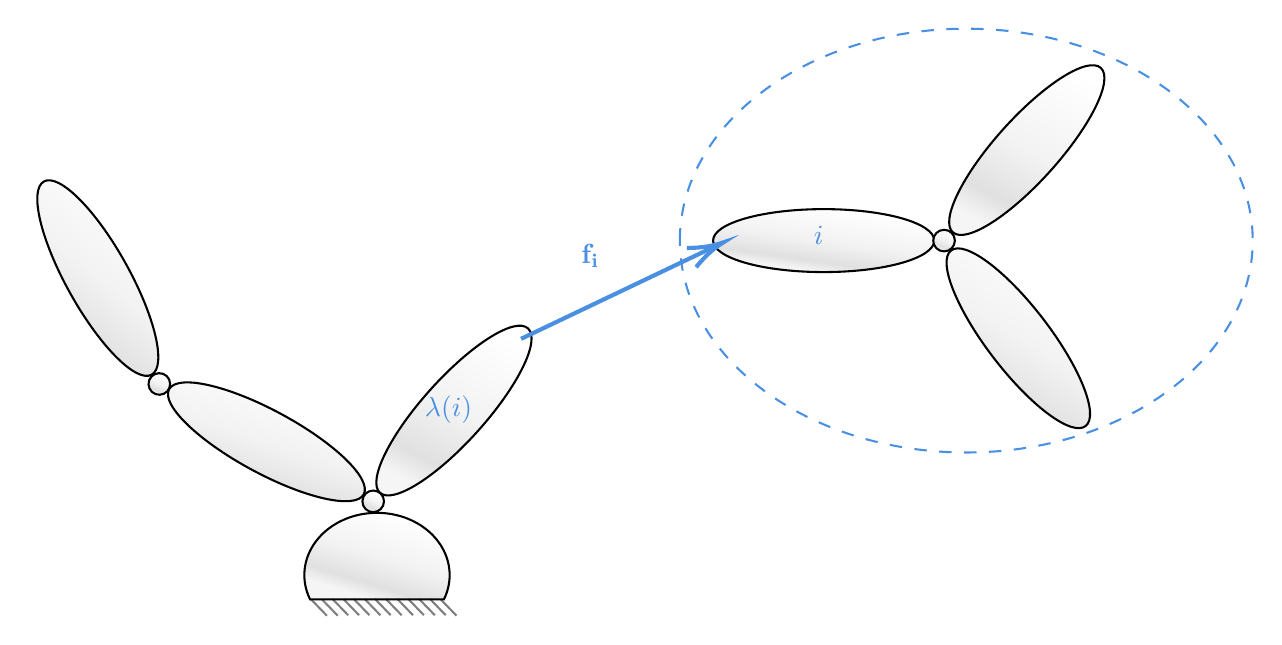
\begin{tikzpicture}[x=0.75pt,y=0.75pt,yscale=-1,xscale=1]
        \path  [shading=_9jgwi88kk,_j7xuj04w0] (382.42,149.33) .. controls (382.42,140.96) and (406.28,134.17) .. (435.71,134.17) .. controls (465.14,134.17) and (489,140.96) .. (489,149.33) .. controls (489,157.71) and (465.14,164.5) .. (435.71,164.5) .. controls (406.28,164.5) and (382.42,157.71) .. (382.42,149.33) -- cycle ; % for fading 
        \draw  [color={rgb, 255:red, 0; green, 0; blue, 0 }  ,draw opacity=1 ][line width=0.75]  (382.42,149.33) .. controls (382.42,140.96) and (406.28,134.17) .. (435.71,134.17) .. controls (465.14,134.17) and (489,140.96) .. (489,149.33) .. controls (489,157.71) and (465.14,164.5) .. (435.71,164.5) .. controls (406.28,164.5) and (382.42,157.71) .. (382.42,149.33) -- cycle ; % for border 
        \path  [shading=_4upvn6zpe,_i29mdsrh8] (569.22,66.11) .. controls (575.45,71.72) and (564.53,93.99) .. (544.84,115.87) .. controls (525.15,137.75) and (504.14,150.94) .. (497.92,145.33) .. controls (491.69,139.73) and (502.61,117.45) .. (522.3,95.58) .. controls (541.99,73.7) and (563,60.51) .. (569.22,66.11) -- cycle ; % for fading 
        \draw  [color={rgb, 255:red, 0; green, 0; blue, 0 }  ,draw opacity=1 ][line width=0.75]  (569.22,66.11) .. controls (575.45,71.72) and (564.53,93.99) .. (544.84,115.87) .. controls (525.15,137.75) and (504.14,150.94) .. (497.92,145.33) .. controls (491.69,139.73) and (502.61,117.45) .. (522.3,95.58) .. controls (541.99,73.7) and (563,60.51) .. (569.22,66.11) -- cycle ; % for border 
        \path  [shading=_feqyochyi,_qh2wfjpes] (488.5,149.33) .. controls (488.5,146.46) and (490.83,144.13) .. (493.71,144.13) .. controls (496.58,144.13) and (498.92,146.46) .. (498.92,149.33) .. controls (498.92,152.21) and (496.58,154.54) .. (493.71,154.54) .. controls (490.83,154.54) and (488.5,152.21) .. (488.5,149.33) -- cycle ; % for fading 
        \draw  [color={rgb, 255:red, 0; green, 0; blue, 0 }  ,draw opacity=1 ][line width=0.75]  (488.5,149.33) .. controls (488.5,146.46) and (490.83,144.13) .. (493.71,144.13) .. controls (496.58,144.13) and (498.92,146.46) .. (498.92,149.33) .. controls (498.92,152.21) and (496.58,154.54) .. (493.71,154.54) .. controls (490.83,154.54) and (488.5,152.21) .. (488.5,149.33) -- cycle ; % for border 
        \path  [shading=_gk602o946,_d10v6gqbc] (293.22,191.61) .. controls (299.45,197.22) and (288.53,219.49) .. (268.84,241.37) .. controls (249.15,263.25) and (228.14,276.44) .. (221.92,270.83) .. controls (215.69,265.23) and (226.61,242.95) .. (246.3,221.08) .. controls (265.99,199.2) and (287,186.01) .. (293.22,191.61) -- cycle ; % for fading 
        \draw  [color={rgb, 255:red, 0; green, 0; blue, 0 }  ,draw opacity=1 ][line width=0.75]  (293.22,191.61) .. controls (299.45,197.22) and (288.53,219.49) .. (268.84,241.37) .. controls (249.15,263.25) and (228.14,276.44) .. (221.92,270.83) .. controls (215.69,265.23) and (226.61,242.95) .. (246.3,221.08) .. controls (265.99,199.2) and (287,186.01) .. (293.22,191.61) -- cycle ; % for border 
        \path  [shading=_l87ke29nk,_8lna51u6m] (213.46,274.96) .. controls (213.46,272.08) and (215.79,269.75) .. (218.67,269.75) .. controls (221.54,269.75) and (223.87,272.08) .. (223.87,274.96) .. controls (223.87,277.83) and (221.54,280.17) .. (218.67,280.17) .. controls (215.79,280.17) and (213.46,277.83) .. (213.46,274.96) -- cycle ; % for fading 
        \draw  [color={rgb, 255:red, 0; green, 0; blue, 0 }  ,draw opacity=1 ][line width=0.75]  (213.46,274.96) .. controls (213.46,272.08) and (215.79,269.75) .. (218.67,269.75) .. controls (221.54,269.75) and (223.87,272.08) .. (223.87,274.96) .. controls (223.87,277.83) and (221.54,280.17) .. (218.67,280.17) .. controls (215.79,280.17) and (213.46,277.83) .. (213.46,274.96) -- cycle ; % for border 
        \path  [shading=_5rkeipgwd,_flvzdphcz] (111.95,213.93) .. controls (104.63,218.01) and (87.08,200.48) .. (72.74,174.78) .. controls (58.4,149.08) and (52.7,124.93) .. (60.02,120.85) .. controls (67.33,116.77) and (84.89,134.3) .. (99.23,160) .. controls (113.57,185.7) and (119.26,209.85) .. (111.95,213.93) -- cycle ; % for fading 
        \draw  [color={rgb, 255:red, 0; green, 0; blue, 0 }  ,draw opacity=1 ][line width=0.75]  (111.95,213.93) .. controls (104.63,218.01) and (87.08,200.48) .. (72.74,174.78) .. controls (58.4,149.08) and (52.7,124.93) .. (60.02,120.85) .. controls (67.33,116.77) and (84.89,134.3) .. (99.23,160) .. controls (113.57,185.7) and (119.26,209.85) .. (111.95,213.93) -- cycle ; % for border 
        \path  [shading=_65i61e978,_lvfzf5nu3] (120.33,220.95) .. controls (124.31,213.58) and (148.53,218.94) .. (174.43,232.93) .. controls (200.32,246.91) and (218.09,264.22) .. (214.11,271.59) .. controls (210.13,278.96) and (185.91,273.6) .. (160.01,259.62) .. controls (134.12,245.63) and (116.35,228.32) .. (120.33,220.95) -- cycle ; % for fading 
        \draw  [color={rgb, 255:red, 0; green, 0; blue, 0 }  ,draw opacity=1 ][line width=0.75]  (120.33,220.95) .. controls (124.31,213.58) and (148.53,218.94) .. (174.43,232.93) .. controls (200.32,246.91) and (218.09,264.22) .. (214.11,271.59) .. controls (210.13,278.96) and (185.91,273.6) .. (160.01,259.62) .. controls (134.12,245.63) and (116.35,228.32) .. (120.33,220.95) -- cycle ; % for border 
        \path  [shading=_h3pg9rf15,_27lop19l0] (115.79,223.61) .. controls (112.92,223.71) and (110.51,221.45) .. (110.42,218.58) .. controls (110.32,215.7) and (112.58,213.3) .. (115.45,213.2) .. controls (118.33,213.11) and (120.73,215.36) .. (120.83,218.24) .. controls (120.92,221.11) and (118.67,223.52) .. (115.79,223.61) -- cycle ; % for fading 
        \draw  [color={rgb, 255:red, 0; green, 0; blue, 0 }  ,draw opacity=1 ][line width=0.75]  (115.79,223.61) .. controls (112.92,223.71) and (110.51,221.45) .. (110.42,218.58) .. controls (110.32,215.7) and (112.58,213.3) .. (115.45,213.2) .. controls (118.33,213.11) and (120.73,215.36) .. (120.83,218.24) .. controls (120.92,221.11) and (118.67,223.52) .. (115.79,223.61) -- cycle ; % for border 
        \path  [shading=_pe1dgwonr,_3yz7x95el] (561.88,238.7) .. controls (555.23,243.8) and (535.33,228.98) .. (517.44,205.61) .. controls (499.55,182.24) and (490.43,159.17) .. (497.09,154.08) .. controls (503.74,148.98) and (523.63,163.8) .. (541.53,187.17) .. controls (559.42,210.54) and (568.53,233.61) .. (561.88,238.7) -- cycle ; % for fading 
        \draw  [color={rgb, 255:red, 0; green, 0; blue, 0 }  ,draw opacity=1 ][line width=0.75]  (561.88,238.7) .. controls (555.23,243.8) and (535.33,228.98) .. (517.44,205.61) .. controls (499.55,182.24) and (490.43,159.17) .. (497.09,154.08) .. controls (503.74,148.98) and (523.63,163.8) .. (541.53,187.17) .. controls (559.42,210.54) and (568.53,233.61) .. (561.88,238.7) -- cycle ; % for border 
        \draw [color={rgb, 255:red, 74; green, 144; blue, 226 }  ,draw opacity=1 ][line width=1.5]    (289.92,196.67) -- (384.71,151.46) ;
        \draw [shift={(387.42,150.17)}, rotate = 154.5] [color={rgb, 255:red, 74; green, 144; blue, 226 }  ,draw opacity=1 ][line width=1.5]    (17.05,-5.13) .. controls (10.84,-2.18) and (5.16,-0.47) .. (0,0) .. controls (5.16,0.47) and (10.84,2.18) .. (17.05,5.13)   ;
        \draw  [color={rgb, 255:red, 74; green, 144; blue, 226 }  ,draw opacity=1 ][dash pattern={on 4.5pt off 4.5pt}] (366.42,149.33) .. controls (366.42,92.95) and (428.2,47.25) .. (504.42,47.25) .. controls (580.63,47.25) and (642.42,92.95) .. (642.42,149.33) .. controls (642.42,205.71) and (580.63,251.42) .. (504.42,251.42) .. controls (428.2,251.42) and (366.42,205.71) .. (366.42,149.33) -- cycle ;
        \path  [shading=_titklq3j6,_hfu6x8eun] (188.28,322.23) .. controls (186.49,318.63) and (185.5,314.66) .. (185.5,310.5) .. controls (185.5,293.93) and (201.17,280.5) .. (220.5,280.5) .. controls (239.83,280.5) and (255.5,293.93) .. (255.5,310.5) .. controls (255.5,314.66) and (254.51,318.63) .. (252.72,322.23) -- cycle ; % for fading 
        \draw   (188.28,322.23) .. controls (186.49,318.63) and (185.5,314.66) .. (185.5,310.5) .. controls (185.5,293.93) and (201.17,280.5) .. (220.5,280.5) .. controls (239.83,280.5) and (255.5,293.93) .. (255.5,310.5) .. controls (255.5,314.66) and (254.51,318.63) .. (252.72,322.23) -- cycle ; % for border 
        \draw [color={rgb, 255:red, 0; green, 0; blue, 0 }  ,draw opacity=0.5 ]   (188.78,322.23) -- (196.36,330.06) ;
        \draw [color={rgb, 255:red, 0; green, 0; blue, 0 }  ,draw opacity=0.5 ]   (251.22,322.23) -- (258.81,330.06) ;
        \draw [color={rgb, 255:red, 0; green, 0; blue, 0 }  ,draw opacity=0.5 ]   (194.03,322.23) -- (201.61,330.06) ;
        \draw [color={rgb, 255:red, 0; green, 0; blue, 0 }  ,draw opacity=0.5 ]   (199.03,321.98) -- (206.61,329.81) ;
        \draw [color={rgb, 255:red, 0; green, 0; blue, 0 }  ,draw opacity=0.5 ]   (204.28,321.98) -- (211.86,329.81) ;
        \draw [color={rgb, 255:red, 0; green, 0; blue, 0 }  ,draw opacity=0.5 ]   (209.28,321.98) -- (216.86,329.81) ;
        \draw [color={rgb, 255:red, 0; green, 0; blue, 0 }  ,draw opacity=0.5 ]   (214.53,321.98) -- (222.11,329.81) ;
        \draw [color={rgb, 255:red, 0; green, 0; blue, 0 }  ,draw opacity=0.5 ]   (219.53,321.98) -- (227.11,329.81) ;
        \draw [color={rgb, 255:red, 0; green, 0; blue, 0 }  ,draw opacity=0.5 ]   (224.78,321.98) -- (232.36,329.81) ;
        \draw [color={rgb, 255:red, 0; green, 0; blue, 0 }  ,draw opacity=0.5 ]   (230.28,321.98) -- (237.86,329.81) ;
        \draw [color={rgb, 255:red, 0; green, 0; blue, 0 }  ,draw opacity=0.5 ]   (235.53,321.98) -- (243.11,329.81) ;
        \draw [color={rgb, 255:red, 0; green, 0; blue, 0 }  ,draw opacity=0.5 ]   (240.78,321.98) -- (248.36,329.81) ;
        \draw [color={rgb, 255:red, 0; green, 0; blue, 0 }  ,draw opacity=0.5 ]   (246.03,321.98) -- (253.61,329.81) ;
        \draw (317.5,149.4) node [anchor=north west][inner sep=0.75pt]  [color={rgb, 255:red, 74; green, 144; blue, 226 }  ,opacity=1 ]  {${\displaystyle \mathbf{f_{i}}}$};
        \draw (429.5,140.9) node [anchor=north west][inner sep=0.75pt]    {$\textcolor[rgb]{0.29,0.56,0.89}{i}$};
        \draw  [draw opacity=0]  (256.6, 230.8) circle [x radius= 21.92, y radius= 14.85]   ;
        \draw (242.1,222.7) node [anchor=north west][inner sep=0.75pt]    {$\textcolor[rgb]{0.29,0.56,0.89}{\lambda }\textcolor[rgb]{0.29,0.56,0.89}{(}\textcolor[rgb]{0.29,0.56,0.89}{i}\textcolor[rgb]{0.29,0.56,0.89}{)}$};
    \end{tikzpicture}
\end{figure}

By diving the kinematic structure in sub-trees, i.e. starting from the leaves and going up to the root, by considering a joint $i$ interacting with the rest of the kinematic chain through an unknown force $\mathbf{f} _i$ defined as:

\begin{equation}
    \mathbf{f} _i = \mathbf{I} _i ^A \mathbf{a} _i + \mathbf{p} ^A _i
\end{equation}

where $\mathbf{I} _i ^A$ is the articulated body inertia, i.e. the inertia felt at the base of the subtree when all its joints are free to move, and $\mathbf{p} ^A _i$ is the associated bias force.

The spatial force acting at joint $i$ and the acceleration of body $i$ are related by:

\begin{equation}
    \boldsymbol{\tau} _i = \mathbf{S} ^T _i \mathbf{f} _i = \mathbf{S} ^T _i (\mathbf{I} _i ^A \mathbf{a} _i + \mathbf{p} ^A _i) = \mathbf{S} ^T _i (\mathbf{I} _i ^A (\mathbf{a} _{\lambda(i)} + \mathbf{S} _i \ddot{\mathbf{q}} _i + \dot{\mathbf{S}} _i \dot{\mathbf{q}} _i)+ \mathbf{p} ^A _i)
\end{equation}

where $\mathbf{S} _i$ is the motion subspace of the $i$-th link, $\mathbf{a} _i$ is the acceleration of the $i$-th link, $\mathbf{a} _{\lambda(i)}$ is the acceleration of the parent link, $\ddot{\mathbf{q}} _i$ is the acceleration of the $i$-th joint, and $\dot{\mathbf{S}} _i$ is the derivative of the motion subspace of the $i$-th link with respect to the joint coordinates.

This yields that once the articulated body inertia and the bais force are know, it is possible to compute the acceleration of each joint independently from the dynamics of the other joints. This is the main advantage of the articulated-body algorithm.

In ABA, first a forward pass is performed to compute the initial articulated body inertia, the initial bias forces and the link velocities, then a backward pass is performed to compute the articulated body inertia and the bias force at each joint and finally a forward pass computes the acceleration of each body in the kinematic chain.
Starting from the Gaussian principle of least constraint, the problem of finding the joint accelerations $\ddot{\mathbf{q}}$ that satisfy the equation of motion:

\begin{equation}
    \mathbf{M} (\mathbf{q}) \ddot{\mathbf{q}} + \mathbf{C} (\mathbf{q}, \dot{\mathbf{q}}) + \mathbf{G} (\mathbf{q}) = \boldsymbol{\tau}
\end{equation}

can be formulated as a constrained optimization problem:

\begin{equation}
    \begin{aligned}
         & \underset{\ddot{\mathbf{q}}}{\text{minimize}}
         &                                               & \frac{1}{2} \ddot{\mathbf{q}} ^T \mathbf{M} (\mathbf{q}) \ddot{\mathbf{q}} + \dot{\mathbf{q}} ^T \mathbf{C} (\mathbf{q}, \dot{\mathbf{q}}) + \mathbf{G} (\mathbf{q}) ^T \ddot{\mathbf{q}} \\
         & \text{subject to}
         &                                               & \mathbf{A} (\mathbf{q}) \ddot{\mathbf{q}} = \mathbf{b} (\mathbf{q}, \dot{\mathbf{q}})
    \end{aligned}
\end{equation}

where $\mathbf{A} (\mathbf{q})$ is the constraint matrix and $\mathbf{b} (\mathbf{q}, \dot{\mathbf{q}})$ is the constraint vector.

The constraint matrix $\mathbf{A} (\mathbf{q})$ is defined as:

\begin{equation}
    \mathbf{A} (\mathbf{q}) = \begin{bmatrix}
        \mathbf{S} _1 ^T \mathbf{M} (\mathbf{q}) \mathbf{S} _1     & \mathbf{S} _1 ^T \mathbf{M} (\mathbf{q}) \mathbf{S} _2     & \dots  & \mathbf{S} _1 ^T \mathbf{M} (\mathbf{q}) \mathbf{S} _{N_B}     \\
        \mathbf{S} _2 ^T \mathbf{M} (\mathbf{q}) \mathbf{S} _1     & \mathbf{S} _2 ^T \mathbf{M} (\mathbf{q}) \mathbf{S} _2     & \dots  & \mathbf{S} _2 ^T \mathbf{M} (\mathbf{q}) \mathbf{S} _{N_B}     \\
        \vdots                                                     & \vdots                                                     & \ddots & \vdots                                                         \\
        \mathbf{S} _{N_B} ^T \mathbf{M} (\mathbf{q}) \mathbf{S} _1 & \mathbf{S} _{N_B} ^T \mathbf{M} (\mathbf{q}) \mathbf{S} _2 & \dots  & \mathbf{S} _{N_B} ^T \mathbf{M} (\mathbf{q}) \mathbf{S} _{N_B} \\
    \end{bmatrix}
\end{equation}

where $\mathbf{S} _i$ is the motion subspace of the $i$-th link. And the constraint vector $\mathbf{b} (\mathbf{q}, \dot{\mathbf{q}})$ is defined as:

\begin{equation}
    \mathbf{b} (\mathbf{q}, \dot{\mathbf{q}}) = \begin{bmatrix}
        \mathbf{S} _1 ^T \mathbf{C} (\mathbf{q}, \dot{\mathbf{q}}) + \mathbf{G} (\mathbf{q})     \\
        \mathbf{S} _2 ^T \mathbf{C} (\mathbf{q}, \dot{\mathbf{q}}) + \mathbf{G} (\mathbf{q})     \\
        \vdots                                                                                   \\
        \mathbf{S} _{N_B} ^T \mathbf{C} (\mathbf{q}, \dot{\mathbf{q}}) + \mathbf{G} (\mathbf{q}) \\
    \end{bmatrix}
\end{equation}

The constraint matrix $\mathbf{A} (\mathbf{q})$ is a symmetric matrix, and it is positive definite if the robot is fully actuated. The constraint vector $\mathbf{b} (\mathbf{q}, \dot{\mathbf{q}})$ is a vector of dimension $N_B$.

Including rotors as extra links in the kinematic chain, and considering that:

- the gearbox inertia is negligible compared to the link inertia;

- the motion subspace of the rotor is the same as the motion subspace of the link to which it is attached scaled by the gear ratio, e.g. the free modes of the rotor are the same as the free modes of the link to which it is attached:

\begin{equation}
    {} ^M \mathbf{S} _i = \boldsymbol{\Gamma} _i \mathbf{S} _i
\end{equation}

- the viscous friction is considered as a dissipative force acting on the link to which the rotor is attached;

% === FIG: Disassembled Motor === %
\begin{figure}
    \centering
    \label{fig:disassembled_motor}
    \caption{Disassembled Motor.}
    \tikzset {_05o9hrnmr/.code = {\pgfsetadditionalshadetransform{ \pgftransformshift{\pgfpoint{0 bp } { 0 bp }  }  \pgftransformrotate{-117 }  \pgftransformscale{2 }  }}}
    \pgfdeclarehorizontalshading{_3050tuc2o}{150bp}{rgb(0bp)=(1,1,1);
        rgb(37.5bp)=(1,1,1);
        rgb(50.08184160505022bp)=(0.95,0.95,0.95);
        rgb(57.64583042689732bp)=(0.88,0.88,0.88);
        rgb(61.33184160505022bp)=(0.96,0.96,0.96);
        rgb(100bp)=(0.96,0.96,0.96)}
    \tikzset {_sukiq91mf/.code = {\pgfsetadditionalshadetransform{ \pgftransformshift{\pgfpoint{0 bp } { 0 bp }  }  \pgftransformrotate{-117 }  \pgftransformscale{2 }  }}}
    \pgfdeclarehorizontalshading{_0sr9vccbw}{150bp}{rgb(0bp)=(1,1,1);
        rgb(37.5bp)=(1,1,1);
        rgb(50.08184160505022bp)=(0.95,0.95,0.95);
        rgb(57.64583042689732bp)=(0.88,0.88,0.88);
        rgb(61.33184160505022bp)=(0.96,0.96,0.96);
        rgb(100bp)=(0.96,0.96,0.96)}
    \tikzset {_g1y39j6wc/.code = {\pgfsetadditionalshadetransform{ \pgftransformshift{\pgfpoint{0 bp } { 0 bp }  }  \pgftransformrotate{-117 }  \pgftransformscale{2 }  }}}
    \pgfdeclarehorizontalshading{_7o0aby0ry}{150bp}{rgb(0bp)=(1,1,1);
        rgb(37.5bp)=(1,1,1);
        rgb(50.08184160505022bp)=(0.95,0.95,0.95);
        rgb(57.64583042689732bp)=(0.88,0.88,0.88);
        rgb(61.33184160505022bp)=(0.96,0.96,0.96);
        rgb(100bp)=(0.96,0.96,0.96)}
    \tikzset {_sx585m017/.code = {\pgfsetadditionalshadetransform{ \pgftransformshift{\pgfpoint{0 bp } { 0 bp }  }  \pgftransformrotate{-117 }  \pgftransformscale{2 }  }}}
    \pgfdeclarehorizontalshading{_vrosuyu06}{150bp}{rgb(0bp)=(1,1,1);
        rgb(37.5bp)=(1,1,1);
        rgb(50.08184160505022bp)=(0.95,0.95,0.95);
        rgb(57.64583042689732bp)=(0.88,0.88,0.88);
        rgb(61.33184160505022bp)=(0.96,0.96,0.96);
        rgb(100bp)=(0.96,0.96,0.96)}
    \tikzset {_xv91ptrsn/.code = {\pgfsetadditionalshadetransform{ \pgftransformshift{\pgfpoint{0 bp } { 0 bp }  }  \pgftransformrotate{-76 }  \pgftransformscale{2 }  }}}
    \pgfdeclarehorizontalshading{_nhul4iann}{150bp}{rgb(0bp)=(0.65,0.81,0.87);
        rgb(37.5bp)=(0.65,0.81,0.87);
        rgb(50.16369138445173bp)=(0.29,0.56,0.89);
        rgb(62.5bp)=(0.29,0.56,0.89);
        rgb(100bp)=(0.29,0.56,0.89)}
    \tikzset{_bbvmxj1ed/.code = {\pgfsetadditionalshadetransform{\pgftransformshift{\pgfpoint{0 bp } { 0 bp }  }  \pgftransformrotate{-76 }  \pgftransformscale{2 } }}}
    \pgfdeclarehorizontalshading{_8bw6u8f13} {150bp} {color(0bp)=(transparent!0);
        color(37.5bp)=(transparent!0);
        color(50.16369138445173bp)=(transparent!84);
        color(62.5bp)=(transparent!35);
        color(100bp)=(transparent!35) }
    \pgfdeclarefading{_wvboa5dv4}{\tikz \fill[shading=_8bw6u8f13,_bbvmxj1ed] (0,0) rectangle (50bp,50bp); }
    \tikzset {_8d2g8fv7x/.code = {\pgfsetadditionalshadetransform{ \pgftransformshift{\pgfpoint{0 bp } { 0 bp }  }  \pgftransformrotate{-117 }  \pgftransformscale{2 }  }}}
    \pgfdeclarehorizontalshading{_jpssjqb7l}{150bp}{rgb(0bp)=(1,1,1);
        rgb(37.5bp)=(1,1,1);
        rgb(50.08184160505022bp)=(0.95,0.95,0.95);
        rgb(57.64583042689732bp)=(0.88,0.88,0.88);
        rgb(61.33184160505022bp)=(0.96,0.96,0.96);
        rgb(100bp)=(0.96,0.96,0.96)}
    \tikzset {_u5ghg7uoq/.code = {\pgfsetadditionalshadetransform{ \pgftransformshift{\pgfpoint{0 bp } { 0 bp }  }  \pgftransformrotate{-117 }  \pgftransformscale{2 }  }}}
    \pgfdeclarehorizontalshading{_12u7vly4x}{150bp}{rgb(0bp)=(1,1,1);
        rgb(37.5bp)=(1,1,1);
        rgb(50.08184160505022bp)=(0.95,0.95,0.95);
        rgb(57.64583042689732bp)=(0.88,0.88,0.88);
        rgb(61.33184160505022bp)=(0.96,0.96,0.96);
        rgb(100bp)=(0.96,0.96,0.96)}
    \tikzset {_v3dyi8y7c/.code = {\pgfsetadditionalshadetransform{ \pgftransformshift{\pgfpoint{0 bp } { 0 bp }  }  \pgftransformrotate{-117 }  \pgftransformscale{2 }  }}}
    \pgfdeclarehorizontalshading{_ww5cykcyv}{150bp}{rgb(0bp)=(1,1,1);
        rgb(37.5bp)=(1,1,1);
        rgb(50.08184160505022bp)=(0.95,0.95,0.95);
        rgb(57.64583042689732bp)=(0.88,0.88,0.88);
        rgb(61.33184160505022bp)=(0.96,0.96,0.96);
        rgb(100bp)=(0.96,0.96,0.96)}
    \tikzset {_xcgjq768j/.code = {\pgfsetadditionalshadetransform{ \pgftransformshift{\pgfpoint{0 bp } { 0 bp }  }  \pgftransformrotate{-76 }  \pgftransformscale{2 }  }}}
    \pgfdeclarehorizontalshading{_ca8b4kvm3}{150bp}{rgb(0bp)=(0.65,0.81,0.87);
        rgb(37.5bp)=(0.65,0.81,0.87);
        rgb(50.16369138445173bp)=(0.29,0.56,0.89);
        rgb(62.5bp)=(0.29,0.56,0.89);
        rgb(100bp)=(0.29,0.56,0.89)}
    \tikzset{_uzy9jcyew/.code = {\pgfsetadditionalshadetransform{\pgftransformshift{\pgfpoint{0 bp } { 0 bp }  }  \pgftransformrotate{-76 }  \pgftransformscale{2 } }}}
    \pgfdeclarehorizontalshading{_gao6d2oe3} {150bp} {color(0bp)=(transparent!0);
        color(37.5bp)=(transparent!0);
        color(50.16369138445173bp)=(transparent!84);
        color(62.5bp)=(transparent!35);
        color(100bp)=(transparent!35) }
    \pgfdeclarefading{_iy7jvpss4}{\tikz \fill[shading=_gao6d2oe3,_uzy9jcyew] (0,0) rectangle (50bp,50bp); }
    \tikzset{every picture/.style={line width=0.75pt}}
    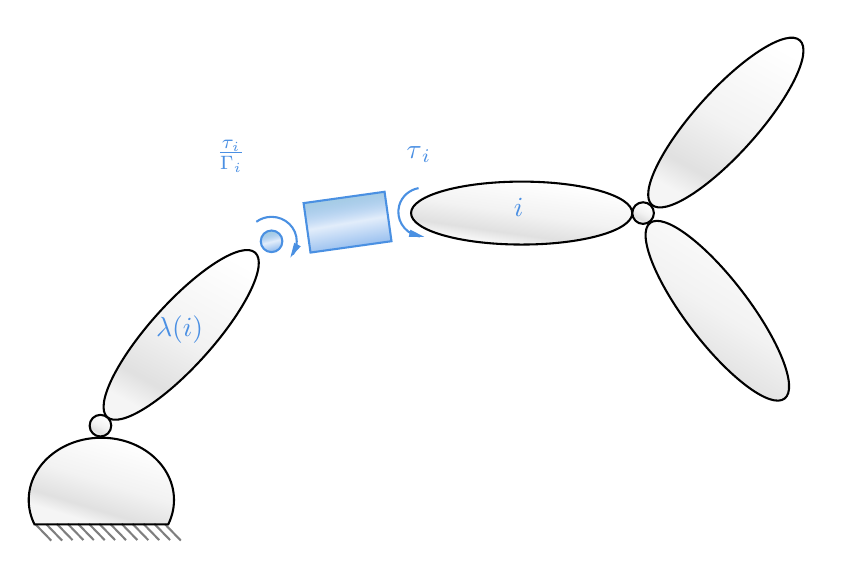
\begin{tikzpicture}[x=0.75pt,y=0.75pt,yscale=-1,xscale=1]
        \path  [shading=_3050tuc2o,_05o9hrnmr] (217.98,165.87) .. controls (217.98,157.49) and (241.84,150.7) .. (271.27,150.7) .. controls (300.71,150.7) and (324.57,157.49) .. (324.57,165.87) .. controls (324.57,174.24) and (300.71,181.03) .. (271.27,181.03) .. controls (241.84,181.03) and (217.98,174.24) .. (217.98,165.87) -- cycle ; % for fading 
        \draw  [color={rgb, 255:red, 0; green, 0; blue, 0 }  ,draw opacity=1 ][line width=0.75]  (217.98,165.87) .. controls (217.98,157.49) and (241.84,150.7) .. (271.27,150.7) .. controls (300.71,150.7) and (324.57,157.49) .. (324.57,165.87) .. controls (324.57,174.24) and (300.71,181.03) .. (271.27,181.03) .. controls (241.84,181.03) and (217.98,174.24) .. (217.98,165.87) -- cycle ; % for border 
        \path  [shading=_0sr9vccbw,_sukiq91mf] (405.29,82.65) .. controls (411.51,88.25) and (400.6,110.53) .. (380.91,132.4) .. controls (361.22,154.28) and (340.21,167.47) .. (333.98,161.87) .. controls (327.76,156.26) and (338.67,133.99) .. (358.36,112.11) .. controls (378.05,90.23) and (399.06,77.04) .. (405.29,82.65) -- cycle ; % for fading 
        \draw  [color={rgb, 255:red, 0; green, 0; blue, 0 }  ,draw opacity=1 ][line width=0.75]  (405.29,82.65) .. controls (411.51,88.25) and (400.6,110.53) .. (380.91,132.4) .. controls (361.22,154.28) and (340.21,167.47) .. (333.98,161.87) .. controls (327.76,156.26) and (338.67,133.99) .. (358.36,112.11) .. controls (378.05,90.23) and (399.06,77.04) .. (405.29,82.65) -- cycle ; % for border 
        \path  [shading=_7o0aby0ry,_g1y39j6wc] (324.57,165.87) .. controls (324.57,162.99) and (326.9,160.66) .. (329.77,160.66) .. controls (332.65,160.66) and (334.98,162.99) .. (334.98,165.87) .. controls (334.98,168.74) and (332.65,171.07) .. (329.77,171.07) .. controls (326.9,171.07) and (324.57,168.74) .. (324.57,165.87) -- cycle ; % for fading 
        \draw  [color={rgb, 255:red, 0; green, 0; blue, 0 }  ,draw opacity=1 ][line width=0.75]  (324.57,165.87) .. controls (324.57,162.99) and (326.9,160.66) .. (329.77,160.66) .. controls (332.65,160.66) and (334.98,162.99) .. (334.98,165.87) .. controls (334.98,168.74) and (332.65,171.07) .. (329.77,171.07) .. controls (326.9,171.07) and (324.57,168.74) .. (324.57,165.87) -- cycle ; % for border 
        \path  [shading=_vrosuyu06,_sx585m017] (142.89,184.95) .. controls (149.11,190.55) and (138.2,212.83) .. (118.51,234.7) .. controls (98.82,256.58) and (77.81,269.77) .. (71.58,264.17) .. controls (65.36,258.56) and (76.27,236.29) .. (95.96,214.41) .. controls (115.65,192.53) and (136.66,179.34) .. (142.89,184.95) -- cycle ; % for fading 
        \draw  [color={rgb, 255:red, 0; green, 0; blue, 0 }  ,draw opacity=1 ][line width=0.75]  (142.89,184.95) .. controls (149.11,190.55) and (138.2,212.83) .. (118.51,234.7) .. controls (98.82,256.58) and (77.81,269.77) .. (71.58,264.17) .. controls (65.36,258.56) and (76.27,236.29) .. (95.96,214.41) .. controls (115.65,192.53) and (136.66,179.34) .. (142.89,184.95) -- cycle ; % for border 
        \path  [shading=_nhul4iann,_xv91ptrsn,path fading= _wvboa5dv4 ,fading transform={xshift=2}] (145.57,179.47) .. controls (145.57,176.59) and (147.9,174.26) .. (150.77,174.26) .. controls (153.65,174.26) and (155.98,176.59) .. (155.98,179.47) .. controls (155.98,182.34) and (153.65,184.67) .. (150.77,184.67) .. controls (147.9,184.67) and (145.57,182.34) .. (145.57,179.47) -- cycle ; % for fading 
        \draw  [color={rgb, 255:red, 74; green, 144; blue, 226 }  ,draw opacity=1 ][line width=0.75]  (145.57,179.47) .. controls (145.57,176.59) and (147.9,174.26) .. (150.77,174.26) .. controls (153.65,174.26) and (155.98,176.59) .. (155.98,179.47) .. controls (155.98,182.34) and (153.65,184.67) .. (150.77,184.67) .. controls (147.9,184.67) and (145.57,182.34) .. (145.57,179.47) -- cycle ; % for border 
        \path  [shading=_jpssjqb7l,_8d2g8fv7x] (63.12,268.29) .. controls (63.12,265.42) and (65.46,263.08) .. (68.33,263.08) .. controls (71.21,263.08) and (73.54,265.42) .. (73.54,268.29) .. controls (73.54,271.17) and (71.21,273.5) .. (68.33,273.5) .. controls (65.46,273.5) and (63.12,271.17) .. (63.12,268.29) -- cycle ; % for fading 
        \draw  [color={rgb, 255:red, 0; green, 0; blue, 0 }  ,draw opacity=1 ][line width=0.75]  (63.12,268.29) .. controls (63.12,265.42) and (65.46,263.08) .. (68.33,263.08) .. controls (71.21,263.08) and (73.54,265.42) .. (73.54,268.29) .. controls (73.54,271.17) and (71.21,273.5) .. (68.33,273.5) .. controls (65.46,273.5) and (63.12,271.17) .. (63.12,268.29) -- cycle ; % for border 
        \path  [shading=_12u7vly4x,_u5ghg7uoq] (397.95,255.24) .. controls (391.3,260.33) and (371.4,245.51) .. (353.51,222.14) .. controls (335.61,198.77) and (326.5,175.7) .. (333.15,170.61) .. controls (339.8,165.52) and (359.7,180.33) .. (377.59,203.7) .. controls (395.48,227.07) and (404.6,250.14) .. (397.95,255.24) -- cycle ; % for fading 
        \draw  [color={rgb, 255:red, 0; green, 0; blue, 0 }  ,draw opacity=1 ][line width=0.75]  (397.95,255.24) .. controls (391.3,260.33) and (371.4,245.51) .. (353.51,222.14) .. controls (335.61,198.77) and (326.5,175.7) .. (333.15,170.61) .. controls (339.8,165.52) and (359.7,180.33) .. (377.59,203.7) .. controls (395.48,227.07) and (404.6,250.14) .. (397.95,255.24) -- cycle ; % for border 
        \path  [shading=_ww5cykcyv,_v3dyi8y7c] (36.54,315.83) .. controls (34.76,312.23) and (33.77,308.26) .. (33.77,304.1) .. controls (33.77,287.53) and (49.44,274.1) .. (68.77,274.1) .. controls (88.1,274.1) and (103.77,287.53) .. (103.77,304.1) .. controls (103.77,308.26) and (102.78,312.23) .. (100.99,315.83) -- cycle ; % for fading 
        \draw   (36.54,315.83) .. controls (34.76,312.23) and (33.77,308.26) .. (33.77,304.1) .. controls (33.77,287.53) and (49.44,274.1) .. (68.77,274.1) .. controls (88.1,274.1) and (103.77,287.53) .. (103.77,304.1) .. controls (103.77,308.26) and (102.78,312.23) .. (100.99,315.83) -- cycle ; % for border 
        \draw [color={rgb, 255:red, 0; green, 0; blue, 0 }  ,draw opacity=0.5 ]   (37.04,315.83) -- (44.63,323.66) ;
        \draw [color={rgb, 255:red, 0; green, 0; blue, 0 }  ,draw opacity=0.5 ]   (99.49,315.83) -- (107.07,323.66) ;
        \draw [color={rgb, 255:red, 0; green, 0; blue, 0 }  ,draw opacity=0.5 ]   (42.29,315.83) -- (49.88,323.66) ;
        \draw [color={rgb, 255:red, 0; green, 0; blue, 0 }  ,draw opacity=0.5 ]   (47.29,315.58) -- (54.88,323.41) ;
        \draw [color={rgb, 255:red, 0; green, 0; blue, 0 }  ,draw opacity=0.5 ]   (52.54,315.58) -- (60.13,323.41) ;
        \draw [color={rgb, 255:red, 0; green, 0; blue, 0 }  ,draw opacity=0.5 ]   (57.54,315.58) -- (65.13,323.41) ;
        \draw [color={rgb, 255:red, 0; green, 0; blue, 0 }  ,draw opacity=0.5 ]   (62.79,315.58) -- (70.38,323.41) ;
        \draw [color={rgb, 255:red, 0; green, 0; blue, 0 }  ,draw opacity=0.5 ]   (67.79,315.58) -- (75.38,323.41) ;
        \draw [color={rgb, 255:red, 0; green, 0; blue, 0 }  ,draw opacity=0.5 ]   (73.04,315.58) -- (80.63,323.41) ;
        \draw [color={rgb, 255:red, 0; green, 0; blue, 0 }  ,draw opacity=0.5 ]   (78.54,315.58) -- (86.13,323.41) ;
        \draw [color={rgb, 255:red, 0; green, 0; blue, 0 }  ,draw opacity=0.5 ]   (83.79,315.58) -- (91.38,323.41) ;
        \draw [color={rgb, 255:red, 0; green, 0; blue, 0 }  ,draw opacity=0.5 ]   (89.04,315.58) -- (96.63,323.41) ;
        \draw [color={rgb, 255:red, 0; green, 0; blue, 0 }  ,draw opacity=0.5 ]   (94.29,315.58) -- (101.88,323.41) ;
        \path  [shading=_ca8b4kvm3,_xcgjq768j,path fading= _iy7jvpss4 ,fading transform={xshift=2}] (166.2,161.07) -- (205.22,155.6) -- (208.56,179.42) -- (169.54,184.89) -- cycle ; % for fading 
        \draw  [color={rgb, 255:red, 74; green, 144; blue, 226 }  ,draw opacity=1 ] (166.2,161.07) -- (205.22,155.6) -- (208.56,179.42) -- (169.54,184.89) -- cycle ; % for border 
        \draw  [draw opacity=0] (143.43,170.08) .. controls (145.47,168.57) and (148.01,167.67) .. (150.77,167.67) .. controls (157.48,167.67) and (162.91,172.95) .. (162.91,179.47) .. controls (162.91,182.49) and (161.74,185.25) .. (159.82,187.34) -- (150.77,179.47) -- cycle ; \draw [color={rgb, 255:red, 74; green, 144; blue, 226 }  ,draw opacity=1 ]   (143.43,170.08) .. controls (145.47,168.57) and (148.01,167.67) .. (150.77,167.67) .. controls (157.48,167.67) and (162.91,172.95) .. (162.91,179.47) .. controls (162.91,181.8) and (162.22,183.97) .. (161.02,185.79) ; \draw [shift={(159.82,187.34)}, rotate = 298.66] [fill={rgb, 255:red, 74; green, 144; blue, 226 }  ,fill opacity=1 ][line width=0.08]  [draw opacity=0] (7.2,-1.8) -- (0,0) -- (7.2,1.8) -- cycle    ;
        \draw  [draw opacity=0] (224.27,177.29) .. controls (223.16,177.3) and (222.03,177.16) .. (220.9,176.85) .. controls (214.43,175.11) and (210.56,168.6) .. (212.25,162.31) .. controls (213.47,157.81) and (217.2,154.64) .. (221.59,153.84) -- (223.97,165.47) -- cycle ; \draw [color={rgb, 255:red, 74; green, 144; blue, 226 }  ,draw opacity=1 ]   (222.27,177.14) .. controls (221.82,177.07) and (221.36,176.98) .. (220.9,176.85) .. controls (214.43,175.11) and (210.56,168.6) .. (212.25,162.31) .. controls (213.47,157.81) and (217.2,154.64) .. (221.59,153.84) ;  \draw [shift={(224.27,177.29)}, rotate = 193.28] [fill={rgb, 255:red, 74; green, 144; blue, 226 }  ,fill opacity=1 ][line width=0.08]  [draw opacity=0] (7.2,-1.8) -- (0,0) -- (7.2,1.8) -- cycle    ;
        \draw (214.4,132.4) node [anchor=north west][inner sep=0.75pt]    {$\textcolor[rgb]{0.29,0.56,0.89}{\boldsymbol{\tau }}\textcolor[rgb]{0.29,0.56,0.89}{_{i}}$};
        \draw (122.8,129.2) node [anchor=north west][inner sep=0.75pt]    {$\textcolor[rgb]{0.29,0.56,0.89}{\frac{\boldsymbol{\tau }_{i}}{\boldsymbol{\Gamma }_{i}}}$};
        \draw (93.6,213.6) node [anchor=north west][inner sep=0.75pt]    {$\textcolor[rgb]{0.29,0.56,0.89}{\lambda }\textcolor[rgb]{0.29,0.56,0.89}{(}\textcolor[rgb]{0.29,0.56,0.89}{i}\textcolor[rgb]{0.29,0.56,0.89}{)}$};
        \draw (266,157.4) node [anchor=north west][inner sep=0.75pt]    {$\textcolor[rgb]{0.29,0.56,0.89}{i}$};
    \end{tikzpicture}
\end{figure}

we can identify the following quantities starting from the equations of motion of the robot:

% === Uncostrained Tree === %
\begin{figure}
    \centering
    \begin{minipage}[b]{0.4\textwidth}
        \caption{Constrained Tree}
        \tikzset {_djnj2rsc4/.code = {\pgfsetadditionalshadetransform{ \pgftransformshift{\pgfpoint{0 bp } { 0 bp }  }  \pgftransformrotate{-117 }  \pgftransformscale{2 }  }}}
        \pgfdeclarehorizontalshading{_idu07h52c}{150bp}{rgb(0bp)=(1,1,1);
            rgb(37.5bp)=(1,1,1);
            rgb(50.08184160505022bp)=(0.95,0.95,0.95);
            rgb(57.64583042689732bp)=(0.88,0.88,0.88);
            rgb(61.33184160505022bp)=(0.96,0.96,0.96);
            rgb(100bp)=(0.96,0.96,0.96)}
        \tikzset {_jsyk5ax1n/.code = {\pgfsetadditionalshadetransform{ \pgftransformshift{\pgfpoint{0 bp } { 0 bp }  }  \pgftransformrotate{-117 }  \pgftransformscale{2 }  }}}
        \pgfdeclarehorizontalshading{_92edxt770}{150bp}{rgb(0bp)=(1,1,1);
            rgb(37.5bp)=(1,1,1);
            rgb(50.08184160505022bp)=(0.95,0.95,0.95);
            rgb(57.64583042689732bp)=(0.88,0.88,0.88);
            rgb(61.33184160505022bp)=(0.96,0.96,0.96);
            rgb(100bp)=(0.96,0.96,0.96)}
        \tikzset {_b0gplq11g/.code = {\pgfsetadditionalshadetransform{ \pgftransformshift{\pgfpoint{0 bp } { 0 bp }  }  \pgftransformrotate{-117 }  \pgftransformscale{2 }  }}}
        \pgfdeclarehorizontalshading{_x22po1g8w}{150bp}{rgb(0bp)=(1,1,1);
            rgb(37.5bp)=(1,1,1);
            rgb(50.08184160505022bp)=(0.95,0.95,0.95);
            rgb(57.64583042689732bp)=(0.88,0.88,0.88);
            rgb(61.33184160505022bp)=(0.96,0.96,0.96);
            rgb(100bp)=(0.96,0.96,0.96)}
        \tikzset {_ivsfd2s3h/.code = {\pgfsetadditionalshadetransform{ \pgftransformshift{\pgfpoint{0 bp } { 0 bp }  }  \pgftransformrotate{-117 }  \pgftransformscale{2 }  }}}
        \pgfdeclarehorizontalshading{_8u84rjokz}{150bp}{rgb(0bp)=(1,1,1);
            rgb(37.5bp)=(1,1,1);
            rgb(50.08184160505022bp)=(0.95,0.95,0.95);
            rgb(57.64583042689732bp)=(0.88,0.88,0.88);
            rgb(61.33184160505022bp)=(0.96,0.96,0.96);
            rgb(100bp)=(0.96,0.96,0.96)}
        \tikzset {_5pcd2h8hv/.code = {\pgfsetadditionalshadetransform{ \pgftransformshift{\pgfpoint{0 bp } { 0 bp }  }  \pgftransformrotate{-117 }  \pgftransformscale{2 }  }}}
        \pgfdeclarehorizontalshading{_lvec74ltu}{150bp}{rgb(0bp)=(1,1,1);
            rgb(37.5bp)=(1,1,1);
            rgb(50.08184160505022bp)=(0.95,0.95,0.95);
            rgb(57.64583042689732bp)=(0.88,0.88,0.88);
            rgb(61.33184160505022bp)=(0.96,0.96,0.96);
            rgb(100bp)=(0.96,0.96,0.96)}
        \tikzset {_37uba45qs/.code = {\pgfsetadditionalshadetransform{ \pgftransformshift{\pgfpoint{0 bp } { 0 bp }  }  \pgftransformrotate{-117 }  \pgftransformscale{2 }  }}}
        \pgfdeclarehorizontalshading{_ik4ni4me2}{150bp}{rgb(0bp)=(1,1,1);
            rgb(37.5bp)=(1,1,1);
            rgb(50.08184160505022bp)=(0.95,0.95,0.95);
            rgb(57.64583042689732bp)=(0.88,0.88,0.88);
            rgb(61.33184160505022bp)=(0.96,0.96,0.96);
            rgb(100bp)=(0.96,0.96,0.96)}
        \tikzset {_z01vd74d5/.code = {\pgfsetadditionalshadetransform{ \pgftransformshift{\pgfpoint{0 bp } { 0 bp }  }  \pgftransformrotate{-117 }  \pgftransformscale{2 }  }}}
        \pgfdeclarehorizontalshading{_rhf2dk4cx}{150bp}{rgb(0bp)=(1,1,1);
            rgb(37.5bp)=(1,1,1);
            rgb(50.08184160505022bp)=(0.95,0.95,0.95);
            rgb(57.64583042689732bp)=(0.88,0.88,0.88);
            rgb(61.33184160505022bp)=(0.96,0.96,0.96);
            rgb(100bp)=(0.96,0.96,0.96)}
        \tikzset {_9fj7ssnk1/.code = {\pgfsetadditionalshadetransform{ \pgftransformshift{\pgfpoint{0 bp } { 0 bp }  }  \pgftransformrotate{-117 }  \pgftransformscale{2 }  }}}
        \pgfdeclarehorizontalshading{_nn6marsz8}{150bp}{rgb(0bp)=(1,1,1);
            rgb(37.5bp)=(1,1,1);
            rgb(50.08184160505022bp)=(0.95,0.95,0.95);
            rgb(57.64583042689732bp)=(0.88,0.88,0.88);
            rgb(61.33184160505022bp)=(0.96,0.96,0.96);
            rgb(100bp)=(0.96,0.96,0.96)}
        \tikzset {_vxd4nfhmk/.code = {\pgfsetadditionalshadetransform{ \pgftransformshift{\pgfpoint{0 bp } { 0 bp }  }  \pgftransformrotate{-117 }  \pgftransformscale{2 }  }}}
        \pgfdeclarehorizontalshading{_be3tjpf6d}{150bp}{rgb(0bp)=(1,1,1);
            rgb(37.5bp)=(1,1,1);
            rgb(50.08184160505022bp)=(0.95,0.95,0.95);
            rgb(57.64583042689732bp)=(0.88,0.88,0.88);
            rgb(61.33184160505022bp)=(0.96,0.96,0.96);
            rgb(100bp)=(0.96,0.96,0.96)}
        \tikzset {_syya3oz6t/.code = {\pgfsetadditionalshadetransform{ \pgftransformshift{\pgfpoint{0 bp } { 0 bp }  }  \pgftransformrotate{-117 }  \pgftransformscale{2 }  }}}
        \pgfdeclarehorizontalshading{_73496xns5}{150bp}{rgb(0bp)=(1,1,1);
            rgb(37.5bp)=(1,1,1);
            rgb(50.08184160505022bp)=(0.95,0.95,0.95);
            rgb(57.64583042689732bp)=(0.88,0.88,0.88);
            rgb(61.33184160505022bp)=(0.96,0.96,0.96);
            rgb(100bp)=(0.96,0.96,0.96)}
        \tikzset{every picture/.style={line width=0.75pt}} %set default line width to 0.75pt        

        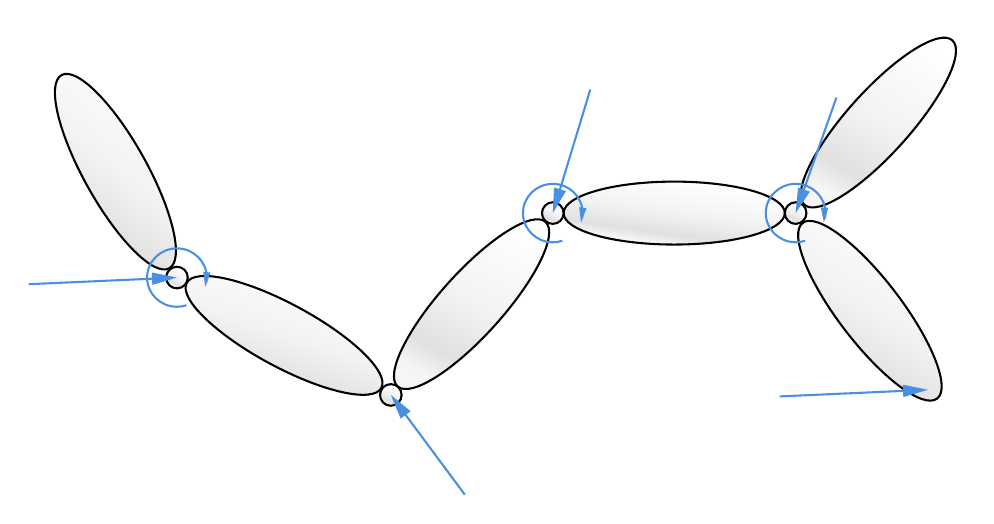
\begin{tikzpicture}[x=0.75pt,y=0.75pt,yscale=-1,xscale=1]
            \path  [shading=_idu07h52c,_djnj2rsc4] (360.92,117.33) .. controls (360.92,108.96) and (384.78,102.17) .. (414.21,102.17) .. controls (443.64,102.17) and (467.5,108.96) .. (467.5,117.33) .. controls (467.5,125.71) and (443.64,132.5) .. (414.21,132.5) .. controls (384.78,132.5) and (360.92,125.71) .. (360.92,117.33) -- cycle ; % for fading 
            \draw  [color={rgb, 255:red, 0; green, 0; blue, 0 }  ,draw opacity=1 ][line width=0.75]  (360.92,117.33) .. controls (360.92,108.96) and (384.78,102.17) .. (414.21,102.17) .. controls (443.64,102.17) and (467.5,108.96) .. (467.5,117.33) .. controls (467.5,125.71) and (443.64,132.5) .. (414.21,132.5) .. controls (384.78,132.5) and (360.92,125.71) .. (360.92,117.33) -- cycle ; % for border 
            \path  [shading=_92edxt770,_jsyk5ax1n] (548.22,34.11) .. controls (554.45,39.72) and (543.53,61.99) .. (523.84,83.87) .. controls (504.15,105.75) and (483.14,118.94) .. (476.92,113.33) .. controls (470.69,107.73) and (481.61,85.45) .. (501.3,63.58) .. controls (520.99,41.7) and (542,28.51) .. (548.22,34.11) -- cycle ; % for fading 
            \draw  [color={rgb, 255:red, 0; green, 0; blue, 0 }  ,draw opacity=1 ][line width=0.75]  (548.22,34.11) .. controls (554.45,39.72) and (543.53,61.99) .. (523.84,83.87) .. controls (504.15,105.75) and (483.14,118.94) .. (476.92,113.33) .. controls (470.69,107.73) and (481.61,85.45) .. (501.3,63.58) .. controls (520.99,41.7) and (542,28.51) .. (548.22,34.11) -- cycle ; % for border 
            \path  [shading=_x22po1g8w,_b0gplq11g] (467.5,117.33) .. controls (467.5,114.46) and (469.83,112.13) .. (472.71,112.13) .. controls (475.58,112.13) and (477.92,114.46) .. (477.92,117.33) .. controls (477.92,120.21) and (475.58,122.54) .. (472.71,122.54) .. controls (469.83,122.54) and (467.5,120.21) .. (467.5,117.33) -- cycle ; % for fading 
            \draw  [color={rgb, 255:red, 0; green, 0; blue, 0 }  ,draw opacity=1 ][line width=0.75]  (467.5,117.33) .. controls (467.5,114.46) and (469.83,112.13) .. (472.71,112.13) .. controls (475.58,112.13) and (477.92,114.46) .. (477.92,117.33) .. controls (477.92,120.21) and (475.58,122.54) .. (472.71,122.54) .. controls (469.83,122.54) and (467.5,120.21) .. (467.5,117.33) -- cycle ; % for border 
            \path  [shading=_8u84rjokz,_ivsfd2s3h] (352.22,121.61) .. controls (358.45,127.22) and (347.53,149.49) .. (327.84,171.37) .. controls (308.15,193.25) and (287.14,206.44) .. (280.92,200.83) .. controls (274.69,195.23) and (285.61,172.95) .. (305.3,151.08) .. controls (324.99,129.2) and (346,116.01) .. (352.22,121.61) -- cycle ; % for fading 
            \draw  [color={rgb, 255:red, 0; green, 0; blue, 0 }  ,draw opacity=1 ][line width=0.75]  (352.22,121.61) .. controls (358.45,127.22) and (347.53,149.49) .. (327.84,171.37) .. controls (308.15,193.25) and (287.14,206.44) .. (280.92,200.83) .. controls (274.69,195.23) and (285.61,172.95) .. (305.3,151.08) .. controls (324.99,129.2) and (346,116.01) .. (352.22,121.61) -- cycle ; % for border 
            \path  [shading=_lvec74ltu,_5pcd2h8hv] (350.5,117.33) .. controls (350.5,114.46) and (352.83,112.13) .. (355.71,112.13) .. controls (358.58,112.13) and (360.92,114.46) .. (360.92,117.33) .. controls (360.92,120.21) and (358.58,122.54) .. (355.71,122.54) .. controls (352.83,122.54) and (350.5,120.21) .. (350.5,117.33) -- cycle ; % for fading 
            \draw  [color={rgb, 255:red, 0; green, 0; blue, 0 }  ,draw opacity=1 ][line width=0.75]  (350.5,117.33) .. controls (350.5,114.46) and (352.83,112.13) .. (355.71,112.13) .. controls (358.58,112.13) and (360.92,114.46) .. (360.92,117.33) .. controls (360.92,120.21) and (358.58,122.54) .. (355.71,122.54) .. controls (352.83,122.54) and (350.5,120.21) .. (350.5,117.33) -- cycle ; % for border 
            \path  [shading=_ik4ni4me2,_37uba45qs] (272.46,204.96) .. controls (272.46,202.08) and (274.79,199.75) .. (277.67,199.75) .. controls (280.54,199.75) and (282.87,202.08) .. (282.87,204.96) .. controls (282.87,207.83) and (280.54,210.17) .. (277.67,210.17) .. controls (274.79,210.17) and (272.46,207.83) .. (272.46,204.96) -- cycle ; % for fading 
            \draw  [color={rgb, 255:red, 0; green, 0; blue, 0 }  ,draw opacity=1 ][line width=0.75]  (272.46,204.96) .. controls (272.46,202.08) and (274.79,199.75) .. (277.67,199.75) .. controls (280.54,199.75) and (282.87,202.08) .. (282.87,204.96) .. controls (282.87,207.83) and (280.54,210.17) .. (277.67,210.17) .. controls (274.79,210.17) and (272.46,207.83) .. (272.46,204.96) -- cycle ; % for border 
            \path  [shading=_rhf2dk4cx,_z01vd74d5] (170.95,143.93) .. controls (163.63,148.01) and (146.08,130.48) .. (131.74,104.78) .. controls (117.4,79.08) and (111.7,54.93) .. (119.02,50.85) .. controls (126.33,46.77) and (143.89,64.3) .. (158.23,90) .. controls (172.57,115.7) and (178.26,139.85) .. (170.95,143.93) -- cycle ; % for fading 
            \draw  [color={rgb, 255:red, 0; green, 0; blue, 0 }  ,draw opacity=1 ][line width=0.75]  (170.95,143.93) .. controls (163.63,148.01) and (146.08,130.48) .. (131.74,104.78) .. controls (117.4,79.08) and (111.7,54.93) .. (119.02,50.85) .. controls (126.33,46.77) and (143.89,64.3) .. (158.23,90) .. controls (172.57,115.7) and (178.26,139.85) .. (170.95,143.93) -- cycle ; % for border 
            \path  [shading=_nn6marsz8,_9fj7ssnk1] (179.33,150.95) .. controls (183.31,143.58) and (207.53,148.94) .. (233.43,162.93) .. controls (259.32,176.91) and (277.09,194.22) .. (273.11,201.59) .. controls (269.13,208.96) and (244.91,203.6) .. (219.01,189.62) .. controls (193.12,175.63) and (175.35,158.32) .. (179.33,150.95) -- cycle ; % for fading 
            \draw  [color={rgb, 255:red, 0; green, 0; blue, 0 }  ,draw opacity=1 ][line width=0.75]  (179.33,150.95) .. controls (183.31,143.58) and (207.53,148.94) .. (233.43,162.93) .. controls (259.32,176.91) and (277.09,194.22) .. (273.11,201.59) .. controls (269.13,208.96) and (244.91,203.6) .. (219.01,189.62) .. controls (193.12,175.63) and (175.35,158.32) .. (179.33,150.95) -- cycle ; % for border 
            \path  [shading=_be3tjpf6d,_vxd4nfhmk] (174.79,153.61) .. controls (171.92,153.71) and (169.51,151.45) .. (169.42,148.58) .. controls (169.32,145.7) and (171.58,143.3) .. (174.45,143.2) .. controls (177.33,143.11) and (179.73,145.36) .. (179.83,148.24) .. controls (179.92,151.11) and (177.67,153.52) .. (174.79,153.61) -- cycle ; % for fading 
            \draw  [color={rgb, 255:red, 0; green, 0; blue, 0 }  ,draw opacity=1 ][line width=0.75]  (174.79,153.61) .. controls (171.92,153.71) and (169.51,151.45) .. (169.42,148.58) .. controls (169.32,145.7) and (171.58,143.3) .. (174.45,143.2) .. controls (177.33,143.11) and (179.73,145.36) .. (179.83,148.24) .. controls (179.92,151.11) and (177.67,153.52) .. (174.79,153.61) -- cycle ; % for border 
            \path  [shading=_73496xns5,_syya3oz6t] (540.88,206.7) .. controls (534.23,211.8) and (514.33,196.98) .. (496.44,173.61) .. controls (478.55,150.24) and (469.43,127.17) .. (476.09,122.08) .. controls (482.74,116.98) and (502.63,131.8) .. (520.53,155.17) .. controls (538.42,178.54) and (547.53,201.61) .. (540.88,206.7) -- cycle ; % for fading 
            \draw  [color={rgb, 255:red, 0; green, 0; blue, 0 }  ,draw opacity=1 ][line width=0.75]  (540.88,206.7) .. controls (534.23,211.8) and (514.33,196.98) .. (496.44,173.61) .. controls (478.55,150.24) and (469.43,127.17) .. (476.09,122.08) .. controls (482.74,116.98) and (502.63,131.8) .. (520.53,155.17) .. controls (538.42,178.54) and (547.53,201.61) .. (540.88,206.7) -- cycle ; % for border 
            \draw [color={rgb, 255:red, 74; green, 144; blue, 226 }  ,draw opacity=1 ]   (103.21,151.6) -- (172.62,148.5) ;
            \draw [shift={(174.62,148.41)}, rotate = 177.44] [fill={rgb, 255:red, 74; green, 144; blue, 226 }  ,fill opacity=1 ][line width=0.08]  [draw opacity=0] (12,-3) -- (0,0) -- (12,3) -- cycle    ;
            \draw [color={rgb, 255:red, 74; green, 144; blue, 226 }  ,draw opacity=1 ]   (373.78,57.81) -- (356.29,115.42) ;
            \draw [shift={(355.71,117.33)}, rotate = 286.89] [fill={rgb, 255:red, 74; green, 144; blue, 226 }  ,fill opacity=1 ][line width=0.08]  [draw opacity=0] (12,-3) -- (0,0) -- (12,3) -- cycle    ;
            \draw [color={rgb, 255:red, 74; green, 144; blue, 226 }  ,draw opacity=1 ]   (465.03,205.67) -- (534.45,202.56) ;
            \draw [shift={(536.44,202.47)}, rotate = 177.44] [fill={rgb, 255:red, 74; green, 144; blue, 226 }  ,fill opacity=1 ][line width=0.08]  [draw opacity=0] (12,-3) -- (0,0) -- (12,3) -- cycle    ;
            \draw [color={rgb, 255:red, 74; green, 144; blue, 226 }  ,draw opacity=1 ]   (492.37,61.67) -- (473.37,115.45) ;
            \draw [shift={(472.71,117.33)}, rotate = 289.46] [fill={rgb, 255:red, 74; green, 144; blue, 226 }  ,fill opacity=1 ][line width=0.08]  [draw opacity=0] (12,-3) -- (0,0) -- (12,3) -- cycle    ;
            \draw  [draw opacity=0] (179.21,161.74) .. controls (177.77,162.22) and (176.23,162.48) .. (174.62,162.48) .. controls (166.68,162.48) and (160.25,156.18) .. (160.25,148.41) .. controls (160.25,140.64) and (166.68,134.34) .. (174.62,134.34) .. controls (182.56,134.34) and (189,140.64) .. (189,148.41) .. controls (189,150) and (188.73,151.53) .. (188.23,152.95) -- (174.62,148.41) -- cycle ; \draw [color={rgb, 255:red, 74; green, 144; blue, 226 }  ,draw opacity=1 ]   (179.21,161.74) .. controls (177.77,162.22) and (176.23,162.48) .. (174.62,162.48) .. controls (166.68,162.48) and (160.25,156.18) .. (160.25,148.41) .. controls (160.25,140.64) and (166.68,134.34) .. (174.62,134.34) .. controls (182.56,134.34) and (189,140.64) .. (189,148.41) .. controls (189,149.31) and (188.91,150.18) .. (188.75,151.04) ; \draw [shift={(188.23,152.95)}, rotate = 276.88] [fill={rgb, 255:red, 74; green, 144; blue, 226 }  ,fill opacity=1 ][line width=0.08]  [draw opacity=0] (7.2,-1.8) -- (0,0) -- (7.2,1.8) -- cycle    ;
            \draw  [draw opacity=0] (360.3,130.67) .. controls (358.86,131.15) and (357.31,131.4) .. (355.71,131.4) .. controls (347.77,131.4) and (341.33,125.1) .. (341.33,117.33) .. controls (341.33,109.56) and (347.77,103.26) .. (355.71,103.26) .. controls (363.65,103.26) and (370.08,109.56) .. (370.08,117.33) .. controls (370.08,118.92) and (369.81,120.45) .. (369.32,121.88) -- (355.71,117.33) -- cycle ; \draw [color={rgb, 255:red, 74; green, 144; blue, 226 }  ,draw opacity=1 ]   (360.3,130.67) .. controls (358.86,131.15) and (357.31,131.4) .. (355.71,131.4) .. controls (347.77,131.4) and (341.33,125.1) .. (341.33,117.33) .. controls (341.33,109.56) and (347.77,103.26) .. (355.71,103.26) .. controls (363.65,103.26) and (370.08,109.56) .. (370.08,117.33) .. controls (370.08,118.23) and (370,119.11) .. (369.83,119.96) ; \draw [shift={(369.32,121.88)}, rotate = 276.88] [fill={rgb, 255:red, 74; green, 144; blue, 226 }  ,fill opacity=1 ][line width=0.08]  [draw opacity=0] (7.2,-1.8) -- (0,0) -- (7.2,1.8) -- cycle    ;
            \draw  [draw opacity=0] (477.3,130.67) .. controls (475.86,131.15) and (474.31,131.4) .. (472.71,131.4) .. controls (464.77,131.4) and (458.33,125.1) .. (458.33,117.33) .. controls (458.33,109.56) and (464.77,103.26) .. (472.71,103.26) .. controls (480.65,103.26) and (487.08,109.56) .. (487.08,117.33) .. controls (487.08,118.92) and (486.81,120.45) .. (486.32,121.88) -- (472.71,117.33) -- cycle ; \draw [color={rgb, 255:red, 74; green, 144; blue, 226 }  ,draw opacity=1 ]   (477.3,130.67) .. controls (475.86,131.15) and (474.31,131.4) .. (472.71,131.4) .. controls (464.77,131.4) and (458.33,125.1) .. (458.33,117.33) .. controls (458.33,109.56) and (464.77,103.26) .. (472.71,103.26) .. controls (480.65,103.26) and (487.08,109.56) .. (487.08,117.33) .. controls (487.08,118.23) and (487,119.11) .. (486.83,119.96) ; \draw [shift={(486.32,121.88)}, rotate = 272.62] [fill={rgb, 255:red, 74; green, 144; blue, 226 }  ,fill opacity=1 ][line width=0.08]  [draw opacity=0] (7.2,-1.8) -- (0,0) -- (7.2,1.8) -- cycle    ;
            \draw [color={rgb, 255:red, 74; green, 144; blue, 226 }  ,draw opacity=1 ]   (313.33,253) -- (278.86,206.56) ;
            \draw [shift={(277.67,204.96)}, rotate = 53.41] [fill={rgb, 255:red, 74; green, 144; blue, 226 }  ,fill opacity=1 ][line width=0.08]  [draw opacity=0] (12,-3) -- (0,0) -- (12,3) -- cycle    ;
        \end{tikzpicture}
    \end{minipage}
    \begin{minipage}[b]{0.4\textwidth}
        \caption{Uncostrained Tree}
        \tikzset {_djnj2rsc4/.code = {\pgfsetadditionalshadetransform{ \pgftransformshift{\pgfpoint{0 bp } { 0 bp }  }  \pgftransformrotate{-117 }  \pgftransformscale{2 }  }}}
        \pgfdeclarehorizontalshading{_idu07h52c}{150bp}{rgb(0bp)=(1,1,1);
            rgb(37.5bp)=(1,1,1);
            rgb(50.08184160505022bp)=(0.95,0.95,0.95);
            rgb(57.64583042689732bp)=(0.88,0.88,0.88);
            rgb(61.33184160505022bp)=(0.96,0.96,0.96);
            rgb(100bp)=(0.96,0.96,0.96)}
        \tikzset {_jsyk5ax1n/.code = {\pgfsetadditionalshadetransform{ \pgftransformshift{\pgfpoint{0 bp } { 0 bp }  }  \pgftransformrotate{-117 }  \pgftransformscale{2 }  }}}
        \pgfdeclarehorizontalshading{_92edxt770}{150bp}{rgb(0bp)=(1,1,1);
            rgb(37.5bp)=(1,1,1);
            rgb(50.08184160505022bp)=(0.95,0.95,0.95);
            rgb(57.64583042689732bp)=(0.88,0.88,0.88);
            rgb(61.33184160505022bp)=(0.96,0.96,0.96);
            rgb(100bp)=(0.96,0.96,0.96)}
        \tikzset {_b0gplq11g/.code = {\pgfsetadditionalshadetransform{ \pgftransformshift{\pgfpoint{0 bp } { 0 bp }  }  \pgftransformrotate{-117 }  \pgftransformscale{2 }  }}}
        \pgfdeclarehorizontalshading{_x22po1g8w}{150bp}{rgb(0bp)=(1,1,1);
            rgb(37.5bp)=(1,1,1);
            rgb(50.08184160505022bp)=(0.95,0.95,0.95);
            rgb(57.64583042689732bp)=(0.88,0.88,0.88);
            rgb(61.33184160505022bp)=(0.96,0.96,0.96);
            rgb(100bp)=(0.96,0.96,0.96)}
        \tikzset {_ivsfd2s3h/.code = {\pgfsetadditionalshadetransform{ \pgftransformshift{\pgfpoint{0 bp } { 0 bp }  }  \pgftransformrotate{-117 }  \pgftransformscale{2 }  }}}
        \pgfdeclarehorizontalshading{_8u84rjokz}{150bp}{rgb(0bp)=(1,1,1);
            rgb(37.5bp)=(1,1,1);
            rgb(50.08184160505022bp)=(0.95,0.95,0.95);
            rgb(57.64583042689732bp)=(0.88,0.88,0.88);
            rgb(61.33184160505022bp)=(0.96,0.96,0.96);
            rgb(100bp)=(0.96,0.96,0.96)}
        \tikzset {_5pcd2h8hv/.code = {\pgfsetadditionalshadetransform{ \pgftransformshift{\pgfpoint{0 bp } { 0 bp }  }  \pgftransformrotate{-117 }  \pgftransformscale{2 }  }}}
        \pgfdeclarehorizontalshading{_lvec74ltu}{150bp}{rgb(0bp)=(1,1,1);
            rgb(37.5bp)=(1,1,1);
            rgb(50.08184160505022bp)=(0.95,0.95,0.95);
            rgb(57.64583042689732bp)=(0.88,0.88,0.88);
            rgb(61.33184160505022bp)=(0.96,0.96,0.96);
            rgb(100bp)=(0.96,0.96,0.96)}
        \tikzset {_37uba45qs/.code = {\pgfsetadditionalshadetransform{ \pgftransformshift{\pgfpoint{0 bp } { 0 bp }  }  \pgftransformrotate{-117 }  \pgftransformscale{2 }  }}}
        \pgfdeclarehorizontalshading{_ik4ni4me2}{150bp}{rgb(0bp)=(1,1,1);
            rgb(37.5bp)=(1,1,1);
            rgb(50.08184160505022bp)=(0.95,0.95,0.95);
            rgb(57.64583042689732bp)=(0.88,0.88,0.88);
            rgb(61.33184160505022bp)=(0.96,0.96,0.96);
            rgb(100bp)=(0.96,0.96,0.96)}
        \tikzset {_z01vd74d5/.code = {\pgfsetadditionalshadetransform{ \pgftransformshift{\pgfpoint{0 bp } { 0 bp }  }  \pgftransformrotate{-117 }  \pgftransformscale{2 }  }}}
        \pgfdeclarehorizontalshading{_rhf2dk4cx}{150bp}{rgb(0bp)=(1,1,1);
            rgb(37.5bp)=(1,1,1);
            rgb(50.08184160505022bp)=(0.95,0.95,0.95);
            rgb(57.64583042689732bp)=(0.88,0.88,0.88);
            rgb(61.33184160505022bp)=(0.96,0.96,0.96);
            rgb(100bp)=(0.96,0.96,0.96)}
        \tikzset {_9fj7ssnk1/.code = {\pgfsetadditionalshadetransform{ \pgftransformshift{\pgfpoint{0 bp } { 0 bp }  }  \pgftransformrotate{-117 }  \pgftransformscale{2 }  }}}
        \pgfdeclarehorizontalshading{_nn6marsz8}{150bp}{rgb(0bp)=(1,1,1);
            rgb(37.5bp)=(1,1,1);
            rgb(50.08184160505022bp)=(0.95,0.95,0.95);
            rgb(57.64583042689732bp)=(0.88,0.88,0.88);
            rgb(61.33184160505022bp)=(0.96,0.96,0.96);
            rgb(100bp)=(0.96,0.96,0.96)}
        \tikzset {_vxd4nfhmk/.code = {\pgfsetadditionalshadetransform{ \pgftransformshift{\pgfpoint{0 bp } { 0 bp }  }  \pgftransformrotate{-117 }  \pgftransformscale{2 }  }}}
        \pgfdeclarehorizontalshading{_be3tjpf6d}{150bp}{rgb(0bp)=(1,1,1);
            rgb(37.5bp)=(1,1,1);
            rgb(50.08184160505022bp)=(0.95,0.95,0.95);
            rgb(57.64583042689732bp)=(0.88,0.88,0.88);
            rgb(61.33184160505022bp)=(0.96,0.96,0.96);
            rgb(100bp)=(0.96,0.96,0.96)}
        \tikzset {_syya3oz6t/.code = {\pgfsetadditionalshadetransform{ \pgftransformshift{\pgfpoint{0 bp } { 0 bp }  }  \pgftransformrotate{-117 }  \pgftransformscale{2 }  }}}
        \pgfdeclarehorizontalshading{_73496xns5}{150bp}{rgb(0bp)=(1,1,1);
            rgb(37.5bp)=(1,1,1);
            rgb(50.08184160505022bp)=(0.95,0.95,0.95);
            rgb(57.64583042689732bp)=(0.88,0.88,0.88);
            rgb(61.33184160505022bp)=(0.96,0.96,0.96);
            rgb(100bp)=(0.96,0.96,0.96)}
        \tikzset{every picture/.style={line width=0.75pt}} %set default line width to 0.75pt        

        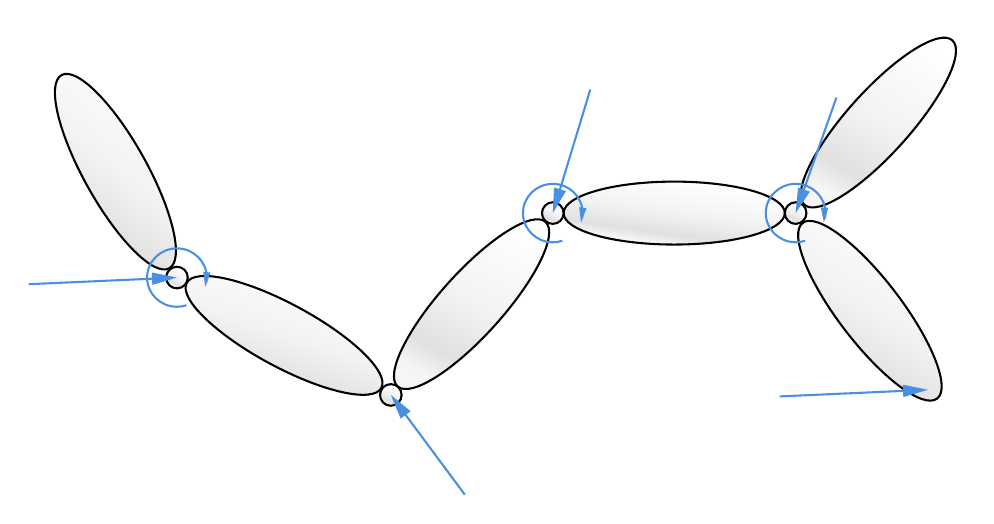
\begin{tikzpicture}[x=0.75pt,y=0.75pt,yscale=-1,xscale=1]
            \path  [shading=_idu07h52c,_djnj2rsc4] (360.92,117.33) .. controls (360.92,108.96) and (384.78,102.17) .. (414.21,102.17) .. controls (443.64,102.17) and (467.5,108.96) .. (467.5,117.33) .. controls (467.5,125.71) and (443.64,132.5) .. (414.21,132.5) .. controls (384.78,132.5) and (360.92,125.71) .. (360.92,117.33) -- cycle ; % for fading 
            \draw  [color={rgb, 255:red, 0; green, 0; blue, 0 }  ,draw opacity=1 ][line width=0.75]  (360.92,117.33) .. controls (360.92,108.96) and (384.78,102.17) .. (414.21,102.17) .. controls (443.64,102.17) and (467.5,108.96) .. (467.5,117.33) .. controls (467.5,125.71) and (443.64,132.5) .. (414.21,132.5) .. controls (384.78,132.5) and (360.92,125.71) .. (360.92,117.33) -- cycle ; % for border 
            \path  [shading=_92edxt770,_jsyk5ax1n] (548.22,34.11) .. controls (554.45,39.72) and (543.53,61.99) .. (523.84,83.87) .. controls (504.15,105.75) and (483.14,118.94) .. (476.92,113.33) .. controls (470.69,107.73) and (481.61,85.45) .. (501.3,63.58) .. controls (520.99,41.7) and (542,28.51) .. (548.22,34.11) -- cycle ; % for fading 
            \draw  [color={rgb, 255:red, 0; green, 0; blue, 0 }  ,draw opacity=1 ][line width=0.75]  (548.22,34.11) .. controls (554.45,39.72) and (543.53,61.99) .. (523.84,83.87) .. controls (504.15,105.75) and (483.14,118.94) .. (476.92,113.33) .. controls (470.69,107.73) and (481.61,85.45) .. (501.3,63.58) .. controls (520.99,41.7) and (542,28.51) .. (548.22,34.11) -- cycle ; % for border 
            \path  [shading=_x22po1g8w,_b0gplq11g] (467.5,117.33) .. controls (467.5,114.46) and (469.83,112.13) .. (472.71,112.13) .. controls (475.58,112.13) and (477.92,114.46) .. (477.92,117.33) .. controls (477.92,120.21) and (475.58,122.54) .. (472.71,122.54) .. controls (469.83,122.54) and (467.5,120.21) .. (467.5,117.33) -- cycle ; % for fading 
            \draw  [color={rgb, 255:red, 0; green, 0; blue, 0 }  ,draw opacity=1 ][line width=0.75]  (467.5,117.33) .. controls (467.5,114.46) and (469.83,112.13) .. (472.71,112.13) .. controls (475.58,112.13) and (477.92,114.46) .. (477.92,117.33) .. controls (477.92,120.21) and (475.58,122.54) .. (472.71,122.54) .. controls (469.83,122.54) and (467.5,120.21) .. (467.5,117.33) -- cycle ; % for border 
            \path  [shading=_8u84rjokz,_ivsfd2s3h] (352.22,121.61) .. controls (358.45,127.22) and (347.53,149.49) .. (327.84,171.37) .. controls (308.15,193.25) and (287.14,206.44) .. (280.92,200.83) .. controls (274.69,195.23) and (285.61,172.95) .. (305.3,151.08) .. controls (324.99,129.2) and (346,116.01) .. (352.22,121.61) -- cycle ; % for fading 
            \draw  [color={rgb, 255:red, 0; green, 0; blue, 0 }  ,draw opacity=1 ][line width=0.75]  (352.22,121.61) .. controls (358.45,127.22) and (347.53,149.49) .. (327.84,171.37) .. controls (308.15,193.25) and (287.14,206.44) .. (280.92,200.83) .. controls (274.69,195.23) and (285.61,172.95) .. (305.3,151.08) .. controls (324.99,129.2) and (346,116.01) .. (352.22,121.61) -- cycle ; % for border 
            \path  [shading=_lvec74ltu,_5pcd2h8hv] (350.5,117.33) .. controls (350.5,114.46) and (352.83,112.13) .. (355.71,112.13) .. controls (358.58,112.13) and (360.92,114.46) .. (360.92,117.33) .. controls (360.92,120.21) and (358.58,122.54) .. (355.71,122.54) .. controls (352.83,122.54) and (350.5,120.21) .. (350.5,117.33) -- cycle ; % for fading 
            \draw  [color={rgb, 255:red, 0; green, 0; blue, 0 }  ,draw opacity=1 ][line width=0.75]  (350.5,117.33) .. controls (350.5,114.46) and (352.83,112.13) .. (355.71,112.13) .. controls (358.58,112.13) and (360.92,114.46) .. (360.92,117.33) .. controls (360.92,120.21) and (358.58,122.54) .. (355.71,122.54) .. controls (352.83,122.54) and (350.5,120.21) .. (350.5,117.33) -- cycle ; % for border 
            \path  [shading=_ik4ni4me2,_37uba45qs] (272.46,204.96) .. controls (272.46,202.08) and (274.79,199.75) .. (277.67,199.75) .. controls (280.54,199.75) and (282.87,202.08) .. (282.87,204.96) .. controls (282.87,207.83) and (280.54,210.17) .. (277.67,210.17) .. controls (274.79,210.17) and (272.46,207.83) .. (272.46,204.96) -- cycle ; % for fading 
            \draw  [color={rgb, 255:red, 0; green, 0; blue, 0 }  ,draw opacity=1 ][line width=0.75]  (272.46,204.96) .. controls (272.46,202.08) and (274.79,199.75) .. (277.67,199.75) .. controls (280.54,199.75) and (282.87,202.08) .. (282.87,204.96) .. controls (282.87,207.83) and (280.54,210.17) .. (277.67,210.17) .. controls (274.79,210.17) and (272.46,207.83) .. (272.46,204.96) -- cycle ; % for border 
            \path  [shading=_rhf2dk4cx,_z01vd74d5] (170.95,143.93) .. controls (163.63,148.01) and (146.08,130.48) .. (131.74,104.78) .. controls (117.4,79.08) and (111.7,54.93) .. (119.02,50.85) .. controls (126.33,46.77) and (143.89,64.3) .. (158.23,90) .. controls (172.57,115.7) and (178.26,139.85) .. (170.95,143.93) -- cycle ; % for fading 
            \draw  [color={rgb, 255:red, 0; green, 0; blue, 0 }  ,draw opacity=1 ][line width=0.75]  (170.95,143.93) .. controls (163.63,148.01) and (146.08,130.48) .. (131.74,104.78) .. controls (117.4,79.08) and (111.7,54.93) .. (119.02,50.85) .. controls (126.33,46.77) and (143.89,64.3) .. (158.23,90) .. controls (172.57,115.7) and (178.26,139.85) .. (170.95,143.93) -- cycle ; % for border 
            \path  [shading=_nn6marsz8,_9fj7ssnk1] (179.33,150.95) .. controls (183.31,143.58) and (207.53,148.94) .. (233.43,162.93) .. controls (259.32,176.91) and (277.09,194.22) .. (273.11,201.59) .. controls (269.13,208.96) and (244.91,203.6) .. (219.01,189.62) .. controls (193.12,175.63) and (175.35,158.32) .. (179.33,150.95) -- cycle ; % for fading 
            \draw  [color={rgb, 255:red, 0; green, 0; blue, 0 }  ,draw opacity=1 ][line width=0.75]  (179.33,150.95) .. controls (183.31,143.58) and (207.53,148.94) .. (233.43,162.93) .. controls (259.32,176.91) and (277.09,194.22) .. (273.11,201.59) .. controls (269.13,208.96) and (244.91,203.6) .. (219.01,189.62) .. controls (193.12,175.63) and (175.35,158.32) .. (179.33,150.95) -- cycle ; % for border 
            \path  [shading=_be3tjpf6d,_vxd4nfhmk] (174.79,153.61) .. controls (171.92,153.71) and (169.51,151.45) .. (169.42,148.58) .. controls (169.32,145.7) and (171.58,143.3) .. (174.45,143.2) .. controls (177.33,143.11) and (179.73,145.36) .. (179.83,148.24) .. controls (179.92,151.11) and (177.67,153.52) .. (174.79,153.61) -- cycle ; % for fading 
            \draw  [color={rgb, 255:red, 0; green, 0; blue, 0 }  ,draw opacity=1 ][line width=0.75]  (174.79,153.61) .. controls (171.92,153.71) and (169.51,151.45) .. (169.42,148.58) .. controls (169.32,145.7) and (171.58,143.3) .. (174.45,143.2) .. controls (177.33,143.11) and (179.73,145.36) .. (179.83,148.24) .. controls (179.92,151.11) and (177.67,153.52) .. (174.79,153.61) -- cycle ; % for border 
            \path  [shading=_73496xns5,_syya3oz6t] (540.88,206.7) .. controls (534.23,211.8) and (514.33,196.98) .. (496.44,173.61) .. controls (478.55,150.24) and (469.43,127.17) .. (476.09,122.08) .. controls (482.74,116.98) and (502.63,131.8) .. (520.53,155.17) .. controls (538.42,178.54) and (547.53,201.61) .. (540.88,206.7) -- cycle ; % for fading 
            \draw  [color={rgb, 255:red, 0; green, 0; blue, 0 }  ,draw opacity=1 ][line width=0.75]  (540.88,206.7) .. controls (534.23,211.8) and (514.33,196.98) .. (496.44,173.61) .. controls (478.55,150.24) and (469.43,127.17) .. (476.09,122.08) .. controls (482.74,116.98) and (502.63,131.8) .. (520.53,155.17) .. controls (538.42,178.54) and (547.53,201.61) .. (540.88,206.7) -- cycle ; % for border 
            \draw [color={rgb, 255:red, 74; green, 144; blue, 226 }  ,draw opacity=1 ]   (103.21,151.6) -- (172.62,148.5) ;
            \draw [shift={(174.62,148.41)}, rotate = 177.44] [fill={rgb, 255:red, 74; green, 144; blue, 226 }  ,fill opacity=1 ][line width=0.08]  [draw opacity=0] (12,-3) -- (0,0) -- (12,3) -- cycle    ;
            \draw [color={rgb, 255:red, 74; green, 144; blue, 226 }  ,draw opacity=1 ]   (373.78,57.81) -- (356.29,115.42) ;
            \draw [shift={(355.71,117.33)}, rotate = 286.89] [fill={rgb, 255:red, 74; green, 144; blue, 226 }  ,fill opacity=1 ][line width=0.08]  [draw opacity=0] (12,-3) -- (0,0) -- (12,3) -- cycle    ;
            \draw [color={rgb, 255:red, 74; green, 144; blue, 226 }  ,draw opacity=1 ]   (465.03,205.67) -- (534.45,202.56) ;
            \draw [shift={(536.44,202.47)}, rotate = 177.44] [fill={rgb, 255:red, 74; green, 144; blue, 226 }  ,fill opacity=1 ][line width=0.08]  [draw opacity=0] (12,-3) -- (0,0) -- (12,3) -- cycle    ;
            \draw [color={rgb, 255:red, 74; green, 144; blue, 226 }  ,draw opacity=1 ]   (492.37,61.67) -- (473.37,115.45) ;
            \draw [shift={(472.71,117.33)}, rotate = 289.46] [fill={rgb, 255:red, 74; green, 144; blue, 226 }  ,fill opacity=1 ][line width=0.08]  [draw opacity=0] (12,-3) -- (0,0) -- (12,3) -- cycle    ;
            \draw  [draw opacity=0] (179.21,161.74) .. controls (177.77,162.22) and (176.23,162.48) .. (174.62,162.48) .. controls (166.68,162.48) and (160.25,156.18) .. (160.25,148.41) .. controls (160.25,140.64) and (166.68,134.34) .. (174.62,134.34) .. controls (182.56,134.34) and (189,140.64) .. (189,148.41) .. controls (189,150) and (188.73,151.53) .. (188.23,152.95) -- (174.62,148.41) -- cycle ; \draw [color={rgb, 255:red, 74; green, 144; blue, 226 }  ,draw opacity=1 ]   (179.21,161.74) .. controls (177.77,162.22) and (176.23,162.48) .. (174.62,162.48) .. controls (166.68,162.48) and (160.25,156.18) .. (160.25,148.41) .. controls (160.25,140.64) and (166.68,134.34) .. (174.62,134.34) .. controls (182.56,134.34) and (189,140.64) .. (189,148.41) .. controls (189,149.31) and (188.91,150.18) .. (188.75,151.04) ; \draw [shift={(188.23,152.95)}, rotate = 276.88] [fill={rgb, 255:red, 74; green, 144; blue, 226 }  ,fill opacity=1 ][line width=0.08]  [draw opacity=0] (7.2,-1.8) -- (0,0) -- (7.2,1.8) -- cycle    ;
            \draw  [draw opacity=0] (360.3,130.67) .. controls (358.86,131.15) and (357.31,131.4) .. (355.71,131.4) .. controls (347.77,131.4) and (341.33,125.1) .. (341.33,117.33) .. controls (341.33,109.56) and (347.77,103.26) .. (355.71,103.26) .. controls (363.65,103.26) and (370.08,109.56) .. (370.08,117.33) .. controls (370.08,118.92) and (369.81,120.45) .. (369.32,121.88) -- (355.71,117.33) -- cycle ; \draw [color={rgb, 255:red, 74; green, 144; blue, 226 }  ,draw opacity=1 ]   (360.3,130.67) .. controls (358.86,131.15) and (357.31,131.4) .. (355.71,131.4) .. controls (347.77,131.4) and (341.33,125.1) .. (341.33,117.33) .. controls (341.33,109.56) and (347.77,103.26) .. (355.71,103.26) .. controls (363.65,103.26) and (370.08,109.56) .. (370.08,117.33) .. controls (370.08,118.23) and (370,119.11) .. (369.83,119.96) ; \draw [shift={(369.32,121.88)}, rotate = 276.88] [fill={rgb, 255:red, 74; green, 144; blue, 226 }  ,fill opacity=1 ][line width=0.08]  [draw opacity=0] (7.2,-1.8) -- (0,0) -- (7.2,1.8) -- cycle    ;
            \draw  [draw opacity=0] (477.3,130.67) .. controls (475.86,131.15) and (474.31,131.4) .. (472.71,131.4) .. controls (464.77,131.4) and (458.33,125.1) .. (458.33,117.33) .. controls (458.33,109.56) and (464.77,103.26) .. (472.71,103.26) .. controls (480.65,103.26) and (487.08,109.56) .. (487.08,117.33) .. controls (487.08,118.92) and (486.81,120.45) .. (486.32,121.88) -- (472.71,117.33) -- cycle ; \draw [color={rgb, 255:red, 74; green, 144; blue, 226 }  ,draw opacity=1 ]   (477.3,130.67) .. controls (475.86,131.15) and (474.31,131.4) .. (472.71,131.4) .. controls (464.77,131.4) and (458.33,125.1) .. (458.33,117.33) .. controls (458.33,109.56) and (464.77,103.26) .. (472.71,103.26) .. controls (480.65,103.26) and (487.08,109.56) .. (487.08,117.33) .. controls (487.08,118.23) and (487,119.11) .. (486.83,119.96) ; \draw [shift={(486.32,121.88)}, rotate = 272.62] [fill={rgb, 255:red, 74; green, 144; blue, 226 }  ,fill opacity=1 ][line width=0.08]  [draw opacity=0] (7.2,-1.8) -- (0,0) -- (7.2,1.8) -- cycle    ;
            \draw [color={rgb, 255:red, 74; green, 144; blue, 226 }  ,draw opacity=1 ]   (313.33,253) -- (278.86,206.56) ;
            \draw [shift={(277.67,204.96)}, rotate = 53.41] [fill={rgb, 255:red, 74; green, 144; blue, 226 }  ,fill opacity=1 ][line width=0.08]  [draw opacity=0] (12,-3) -- (0,0) -- (12,3) -- cycle    ;
        \end{tikzpicture}
    \end{minipage}

\end{figure}

\begin{equation}
    \mathbf{a} ^{uncostrained} _i = (\mathbf{I} ^A _i) ^{-1}(\mathbf{S} _i \boldsymbol{\tau} _i - \mathbf{p} ^A _i)
\end{equation}

in a similar fashion, the rotor feels the same force, but the torque is scaled by the gear ratio:

\begin{equation}
    \mathbf{a} ^{uncostrained} _{R _i} = (\mathbf{I} ^M _i) ^{-1}(\mathbf{S} _i \frac{\boldsymbol{\tau} _i}{\boldsymbol{\Gamma} _i} - \mathbf{p} ^M _i)
\end{equation}

where $\mathbf{I} ^M _i$ is the inertia of the rotor, $\mathbf{p} ^M _i$ is the bias force of the rotor defined as $\mathbf{p} ^M _i = {} ^M \mathbf{v} _i\times ^* \mathbf{I} ^M _i {} ^M \mathbf{v} _i$, where ${} ^M \mathbf{v} = \mathbf{v} _{\lambda (i)} + {} ^M \mathbf{S} _i \dot{\mathbf{q}} _i$ and $\boldsymbol{\Gamma} _i$ is the gear ratio.

In the constrained case instead, the admissible accelerations of each joint are limited by the acceleration of the rest of the kinematic chain.


\begin{equation}
    \mathbf{a} ^{constrained} _i = \mathbf{S} _i \ddot{\mathbf{q}} _i + \underbrace{\mathbf{v} _i \times ^* \mathbf{S} _i \dot{\mathbf{q}}} _{\mathbf{c} _i}
\end{equation}

where $\mathbf{c} _i$ is the Coriolis acceleration. The equation for the rotor is then:

\begin{equation}
    {} ^M \mathbf{a} ^{constrained} _i = {} ^M \mathbf{S} _i \ddot{\mathbf{q}} _i + \underbrace{{} ^M \mathbf{v} _i \times ^* {} ^M\mathbf{S} _i \dot{\mathbf{q}}} _{{} ^M \mathbf{c} _i}
\end{equation}

This yields, in term of the Gauss principle of least constraint:

\begin{align}
    \underset{\ddot{\mathbf{q}}}{\arg \min} & \qquad (\mathbf{a} _i - \mathbf{a} _i ^{uc}) \mathbf{I} ^A _i (\mathbf{a} _i - \mathbf{a} _i ^{uc}) + ({} ^M \mathbf{a} _i - {} ^M \mathbf{a} _i ^{uc}) \mathbf{I} ^M _i ({} ^M \mathbf{a} _i - {} ^M \mathbf{a} _i ^{uc}) \nonumber           \\
    \text{where }                           & \qquad \mathbf{a} _i = \mathbf{a} _{\lambda (i)} + \mathbf{S} _i \ddot{\mathbf{q}} _i + \mathbf{c} _i \text{ and } {} ^M \mathbf{a} _i = \mathbf{a} _{\lambda (i)} + {} ^M  \mathbf{S} _i \ddot{\mathbf{q}} _i + {} ^M \mathbf{c} _i \nonumber \\
\end{align}

The objective function can be then expanded as:

\begin{equation}
    J = \mathbf{a} ^T _i \mathbf{I} ^A _i \mathbf{a} _i - 2\mathbf{a} ^T _i \mathbf{I} ^a _i \mathbf{a} ^{uc} _i + (\mathbf{a} ^{uc} _i) ^T \mathbf{I} ^a _i \mathbf{a} ^{uc} _i + {} ^M \mathbf{a} ^T _i \mathbf{I} ^M _i {} ^M \mathbf{a} _i - 2 {} ^M \mathbf{a} ^T _i \mathbf{I} ^M _i {} ^M \mathbf{a} ^{uc} _i + ({} ^M \mathbf{a} ^{uc} _i) ^T \mathbf{I} ^M _i {} ^M \mathbf{a} ^{uc} _i
\end{equation}

as any term that is not quadratic in $\ddot{\mathbf{q}}$ is zero. The objective function can be then rewritten as:

\begin{equation}
    J _1 = \mathbf{a} ^T _i \mathbf{I} ^A _i \mathbf{a} _i - 2\mathbf{a} ^T _i \mathbf{I} ^a _i \mathbf{a} ^{uc} _i
\end{equation}

and

\begin{equation}
    J _2 = {} ^M \mathbf{a} ^T _i \mathbf{I} ^M _i {} ^M \mathbf{a} _i - 2 {} ^M \mathbf{a} ^T _i \mathbf{I} ^M _i {} ^M \mathbf{a} ^{uc} _i
\end{equation}

substituting the constrainst in the objective function, removing terms not depending on $\ddot{\mathbf{q}}$ and taking the gradient, the following equation is obtained:

\begin{align}
    \frac{\partial J _1}{\partial \ddot{\mathbf{q}} _i} & = 2 \mathbf{S} ^T _i \mathbf{I} ^A _i \mathbf{S} _i \ddot{\mathbf{q}} _i + 2 \mathbf{S} ^T _i \mathbf{I} ^A _i (\mathbf{a} _{\lambda (i)} + \mathbf{c} _i) - 2 \mathbf{S} ^T _i \mathbf{I} ^A _i \mathbf{a} ^{uc} _i \nonumber                                        \\
    \frac{\partial J _2}{\partial \ddot{\mathbf{q}} _i} & = 2 {} ^M \mathbf{S} ^T _i \mathbf{I} ^M _i {} ^M \mathbf{S} _i \ddot{\mathbf{q}} _i + 2 {} ^M  \mathbf{S} ^T _i \mathbf{I} ^M _i (\mathbf{a} _{\lambda (i)} + {} ^M  \mathbf{c} _i) - 2 {} ^M \mathbf{S} ^T _i \mathbf{I} ^M _i {} ^M \mathbf{a} ^{uc} _i  \nonumber
\end{align}

Adding up the two terms and defining for compactness:

\begin{equation}
    \mathbf{D} _i = \mathbf{S} ^T _i \mathbf{I} ^A _i \mathbf{S} _i + {} ^M \mathbf{S} ^T _i \mathbf{I} ^M _i {} ^M \mathbf{S} _i
\end{equation}

we get to:

\begin{equation}
    \ddot{\mathbf{q}} _i = \mathbf{D} _i ^{-1} (\mathbf{S} ^T _i \mathbf{I} ^A _i (\mathbf{a} _{\lambda (i)} + \mathbf{c} _i - \mathbf{a} ^{uc} _i) + {} ^M \mathbf{S} ^T _i \mathbf{I} ^M _i ( \mathbf{a} _{\lambda (i)} + {} ^M \mathbf{c} _i - {} ^M \mathbf{a} ^{uc} _i))
\end{equation}

\begin{algorithm}[H]
    \caption{Articulated Body Algorithm}
    \label{alg:aba}
    \begin{algorithmic}[1]
        \FOR{$i = 1 \text{ to } N_B$}
        \STATE $[\mathbf{X}_J, \mathbf{S}_i] = \text{jcalc}(\text{jtype}(i), \dot{\mathbf{q}}_i)$
        \STATE $\color{webgreen}{[{} ^R\mathbf{X}_J, {} ^R\mathbf{S}_i] = \text{jcalc}(\text{jtype}(i), \dot{\mathbf{q}}_i \boldsymbol{\Gamma} _i)}$
        \STATE $\mathrm{\mathbf{v}}_J = \mathbf{S}_i \dot{\mathbf{q}}_i$
        \STATE $\color{webgreen}{\mathrm{{} ^R\mathbf{v}}_J = {} ^R\mathbf{S}_i \dot{\mathbf{q}}_i}$
        \STATE $^i\mathbf{X}_{\lambda(i)} = \mathbf{X}_J\mathbf{X}_T (i)$
        \IF{$\lambda_i = 0$}
        \STATE $\mathrm{\mathbf{v}}_i = \mathrm{\mathbf{v}}_J$
        \STATE $\color{webgreen}{{}^R\mathrm{\mathbf{v}}_i = {}^R\mathrm{\mathbf{v}}_J}$
        \STATE $\mathbf{c}_i \color{webgreen}{,{}^R\mathbf{c}_i} = \mathbf{0}$
        \ELSE
        \STATE $\mathrm{\mathbf{v}}_i = {}^i\mathbf{X} _{\lambda(i)}\mathrm{\mathbf{v}}_{\lambda(i)} + \mathrm{\mathbf{v}}_J$
        \STATE $\color{webgreen}{{}^R\mathrm{\mathbf{v}}_i =  {}^i\mathbf{X} _{\lambda(i)} {}^R\mathrm{\mathbf{v}}_{\lambda(i)} + {}^R\mathrm{\mathbf{v}}_J}$
        \STATE $\mathbf{c}_i = \mathrm{\mathbf{v}}_i \times ^* \mathrm{\mathbf{v}}_J$
        \STATE $\color{webgreen}{{}^R\mathbf{c}_i = {}^R\mathrm{\mathbf{v}}_i \times ^* {}^R\mathrm{\mathbf{v}}_J}$
        \ENDIF
        % \STATE $\mathbf{I}_i ^A = \mathbf{I}_i$
        \STATE $\mathbf{p}_i ^A = \mathrm{\mathbf{v}}_i \times^* \mathbf{I}_i ^A \mathrm{\mathbf{v}}_i - ^i\mathbf{X} _0 ^* f ^* _i $
        \STATE \color{webgreen}{$\mathbf{p}_i ^R = {} ^R\mathrm{\mathbf{v}}_i \times^* \mathbf{I}_i ^R\mathrm{\mathbf{v}}_i - \boldsymbol{\Gamma} ^{-T}\mathbf{K}_v \boldsymbol{\Gamma} ^{-1} \mathbf{\dot{q}}$}
        \ENDFOR

        % Pass 2
        \FOR{$i = N_B \text{ to } 1$}
        \STATE $\mathbf{U}_i = \mathbf{I}_i ^A \mathbf{S}_i$
        \STATE $\color{webgreen}{{}^R\mathbf{U}_i = \mathbf{I}_i ^R {}^R\mathbf{S}_i}$
        \STATE $\mathbf{D} _i = \mathbf{S} ^T _i  {} \mathbf{U} _i \mathbf{S} _i \textcolor{webgreen}{+ {} ^M\mathbf{S} ^T _i  {} ^M\mathbf{U} _i {} ^M\mathbf{S} _i}$
        \STATE $\mathbf{u}_i = \boldsymbol{\tau}_i - \mathbf{S}_i\mathbf{p}_i^A$
        \STATE $\color{webgreen}{{}^R\mathbf{u}_i = \boldsymbol{\Gamma}^{-T}\boldsymbol{\tau}_i - {}^R\mathbf{S}_i\mathbf{p}_i^R}$
        \IF{$\lambda_i \neq 0$}
        \STATE $\mathbf{I} ^A = \mathbf{I} ^A _{\lambda (i)} + {} ^i X _{\lambda (i)} ^T (\mathbf{I} _i ^A + \textcolor{webgreen}{\mathbf{I} _i ^M } - {}  \mathbf{U} _i  \mathbf{D} ^{-1} _i  {}  \mathbf{U} ^T _i \textcolor{webgreen}{- {} ^M \mathbf{U} _i  \mathbf{D} ^{-1} _i {} ^M \mathbf{U} ^T _i}) {} ^i X _{\lambda (i)} $
        \STATE $\mathbf{p} ^A = \mathbf{p} ^A _{\lambda (i)} + {} ^i X _{\lambda (i)} ^T (\mathbf{p} ^A_i + \textcolor{webgreen}{\mathbf{p} ^M_i } + \mathbf{I} ^A _{\lambda (i)}  \mathbf{c}_i + \textcolor{webgreen}{\mathbf{I} {} ^M _i \mathbf{c} ^M _i }+ {}  \mathbf{U} _i \mathbf{D} ^{-1} _i {} \mathbf{u} _i + \textcolor{webgreen}{{} ^M \mathbf{U} _i \mathbf{D} ^{-1} _i {} ^M\mathbf{u} _i}) $
        \ENDIF
        \ENDFOR

        % Pass 3
        \FOR{$i = 1 \text{ to } N_B$}
        \IF{$\lambda_i = 0$}
        \STATE $\mathbf{a}' = -\mathbf{a}_g$
        \ELSE
        \STATE $\mathbf{a}' = {}^{\lambda(i)}\mathbf{X}_i \mathbf{a}_{\lambda(i)}$
        \STATE $\ddot{\mathbf{q}}_i = \mathbf{D}^{-1} (\mathbf{u}_i \textcolor{webgreen}{+ {}^R\mathbf{u}_i }- (\mathbf{U}_i^T + \textcolor{webgreen}{{}^R\mathbf{U}_i^T})\mathbf{a}')$
        \STATE $\mathbf{a}_i = \mathbf{a}' + \mathbf{S}_i\mathbf{\ddot{q}}_i + \mathbf{c} _i$
        \ENDIF
        \ENDFOR
    \end{algorithmic}
\end{algorithm}
